\newsection
\section*{ПРИЛОЖЕНИЕ А \\ Представление графического материала}
\addcontentsline{toc}{section}{ПРИЛОЖЕНИЕ А Представление графического материала}

Графический материал, выполненный на отдельных листах, изображен на рисунках A.1-A.12
%\begin{itemize}
	%\item А.1 - Сведения о ВКРБ.
	%\item A.2 - Цель и задачи разработки.
	%\item A.3 - Концептуальная модель сайта.
	%\item A.4 - Диаграмма прецедентов.
	%\item A.5 - Схема базы данных.
	%\item A.6 - Диаграмма развертывания.
	%\item A.7 - Диаграмма классов.
	%\item A.8 - Дизайн интерфейса. Веб-страница авторизации.
	%\item A.9 - Дизайн интерфейса. Веб-страница регистрации пациента.
	%\item A.10 - Дизайн интерфейса. Веб-страница регистрации врача.
	%\item A.11 - Дизайн интерфейса. Веб-страница для ввода результатов анализа крови.
	%\item А.12 - Заключение.
%\end{itemize} 

\renewcommand{\thefigure}{А.\arabic{figure}} % шаблон номера рисунков


\begin{figure}
  \begin{adjustbox}{addcode={\begin{minipage}{\width}}{\caption{%
          Сведения о ВКРБ
      }\end{minipage}},rotate=90,center}
    
\includegraphics[width=1.3\linewidth]{плакат1.png}
  \end{adjustbox}
  \label{pl1:image}      
\end{figure}

\begin{figure}
  \begin{adjustbox}{addcode={\begin{minipage}{\width}}{\caption{%
          Цель и задачи работы
      }\end{minipage}},rotate=90,center}
    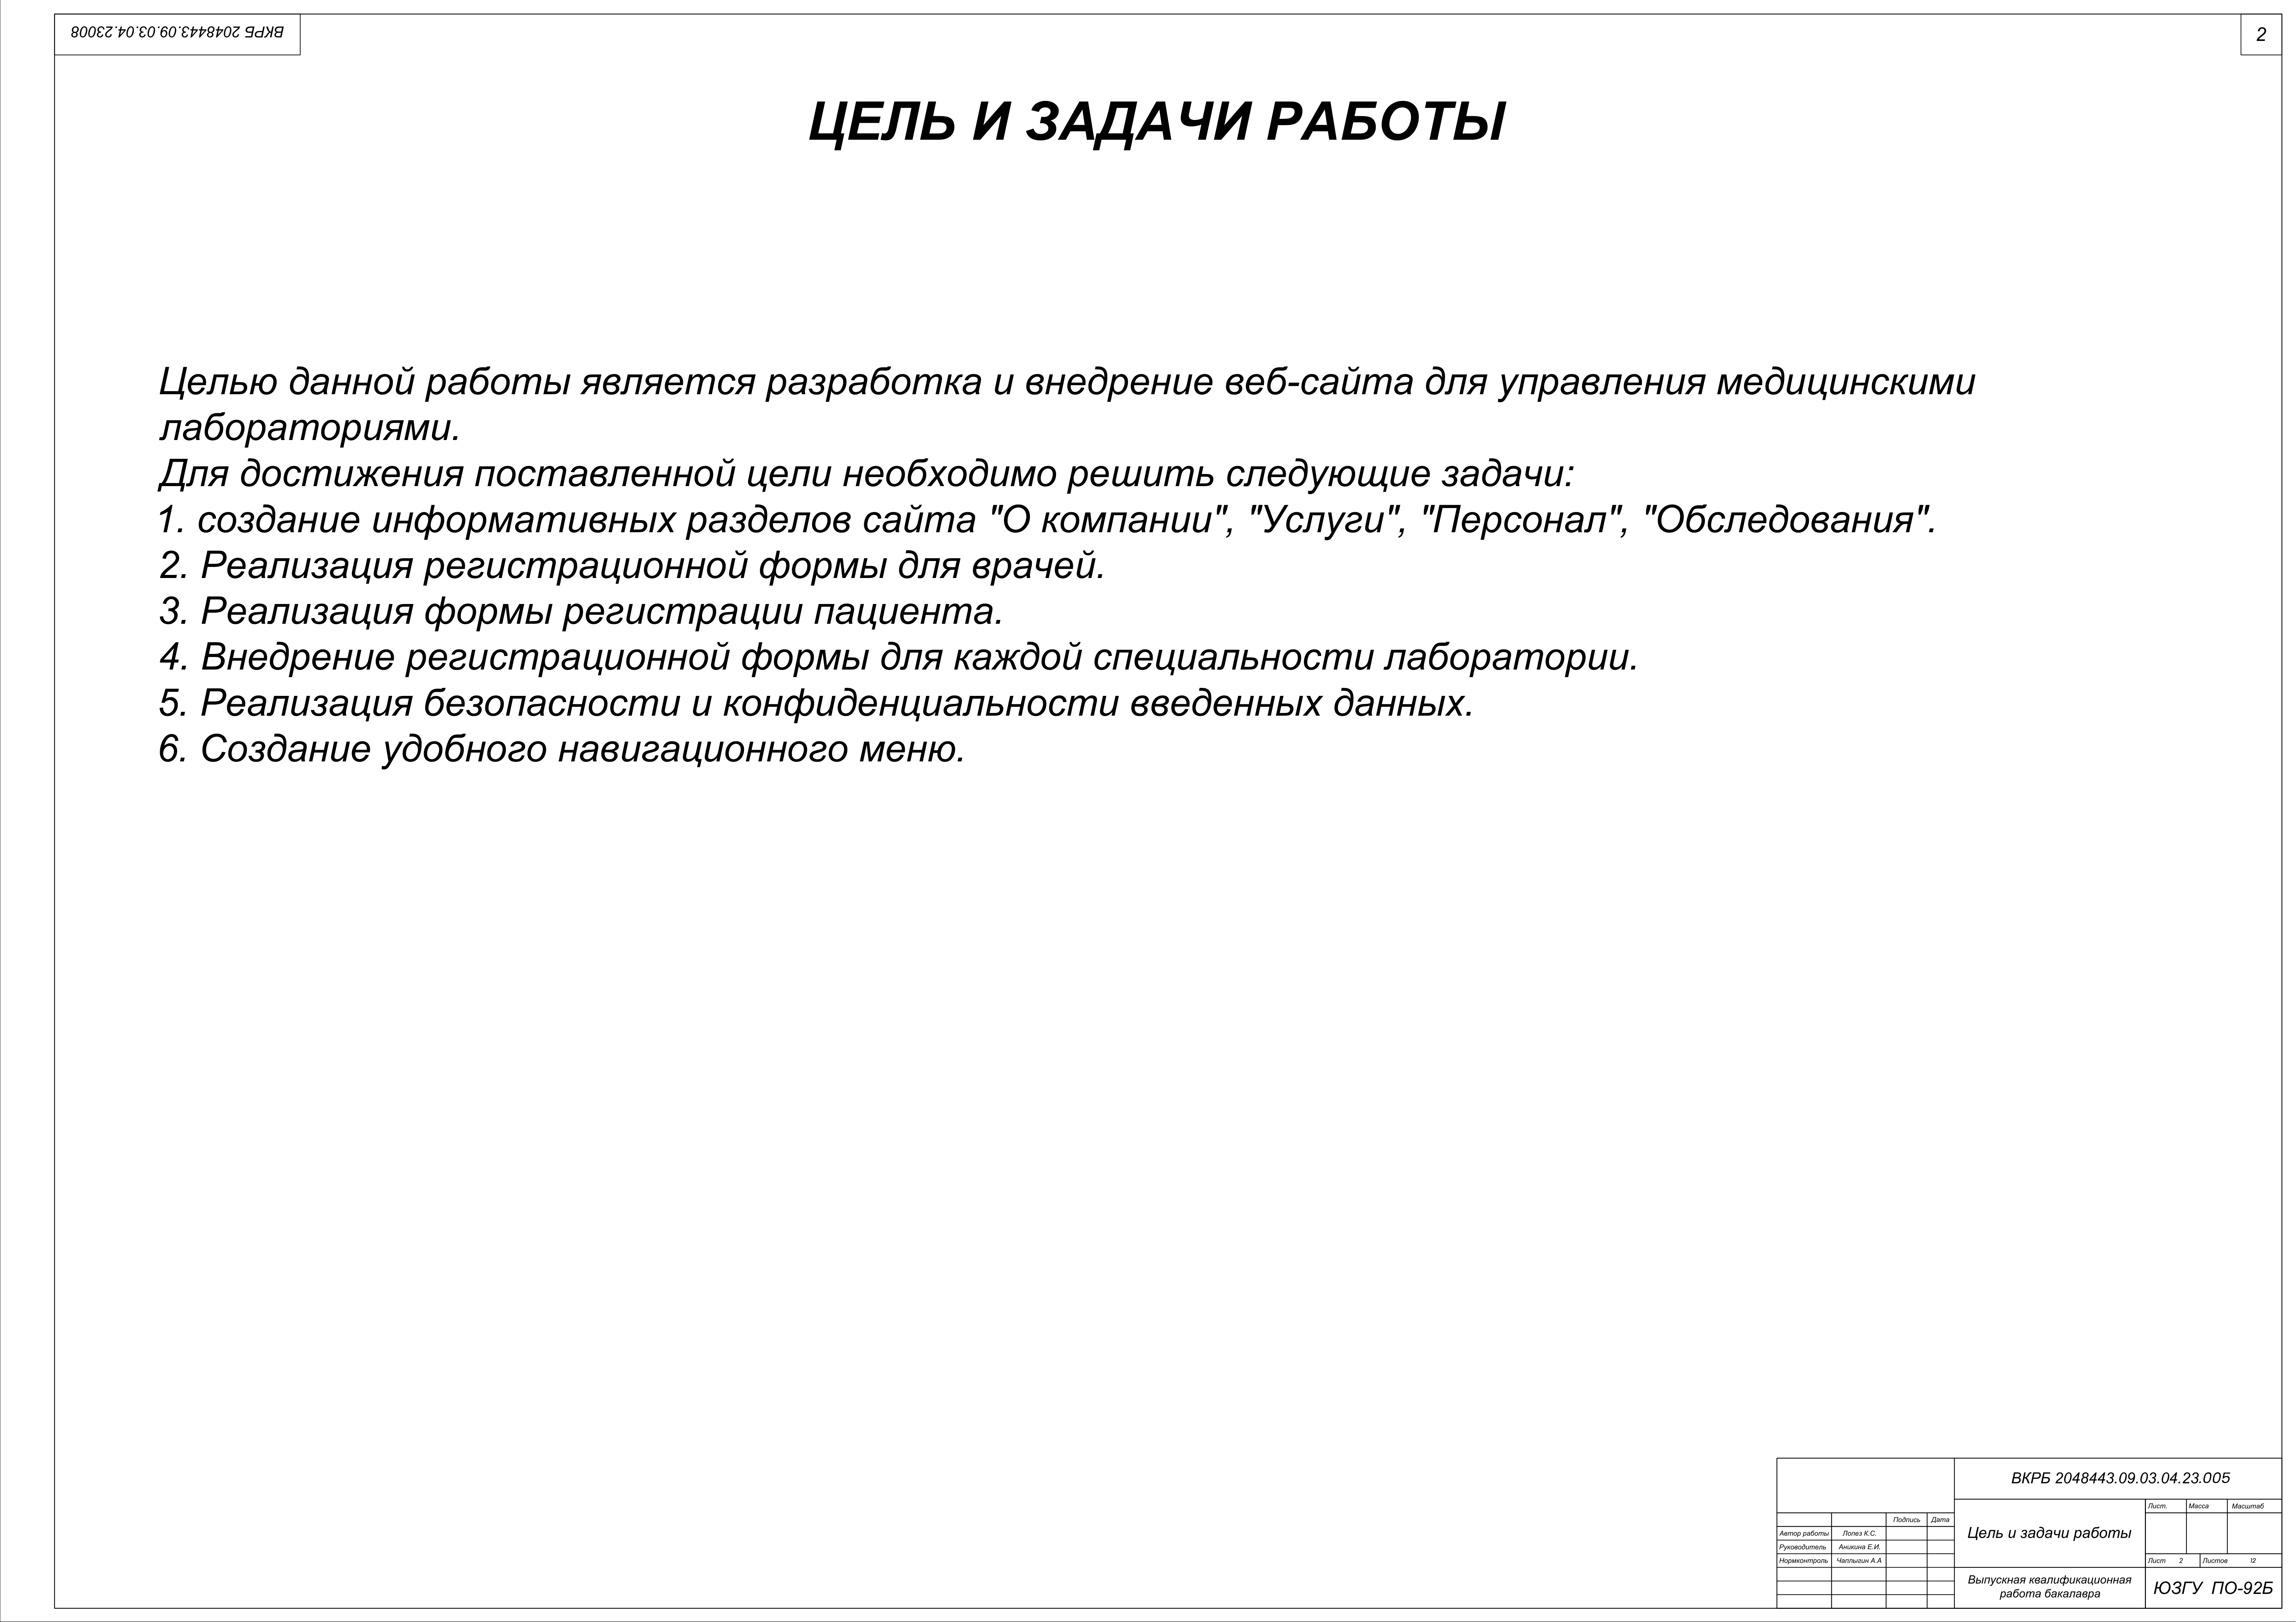
\includegraphics[width=1.3\linewidth]{плакат2.png}
  \end{adjustbox}
  \label{pl2:image}      
\end{figure}

\begin{figure}
  \begin{adjustbox}{addcode={\begin{minipage}{\width}}{\caption{%
          Концептуальная модель сайта
      }\end{minipage}},rotate=90,center}
    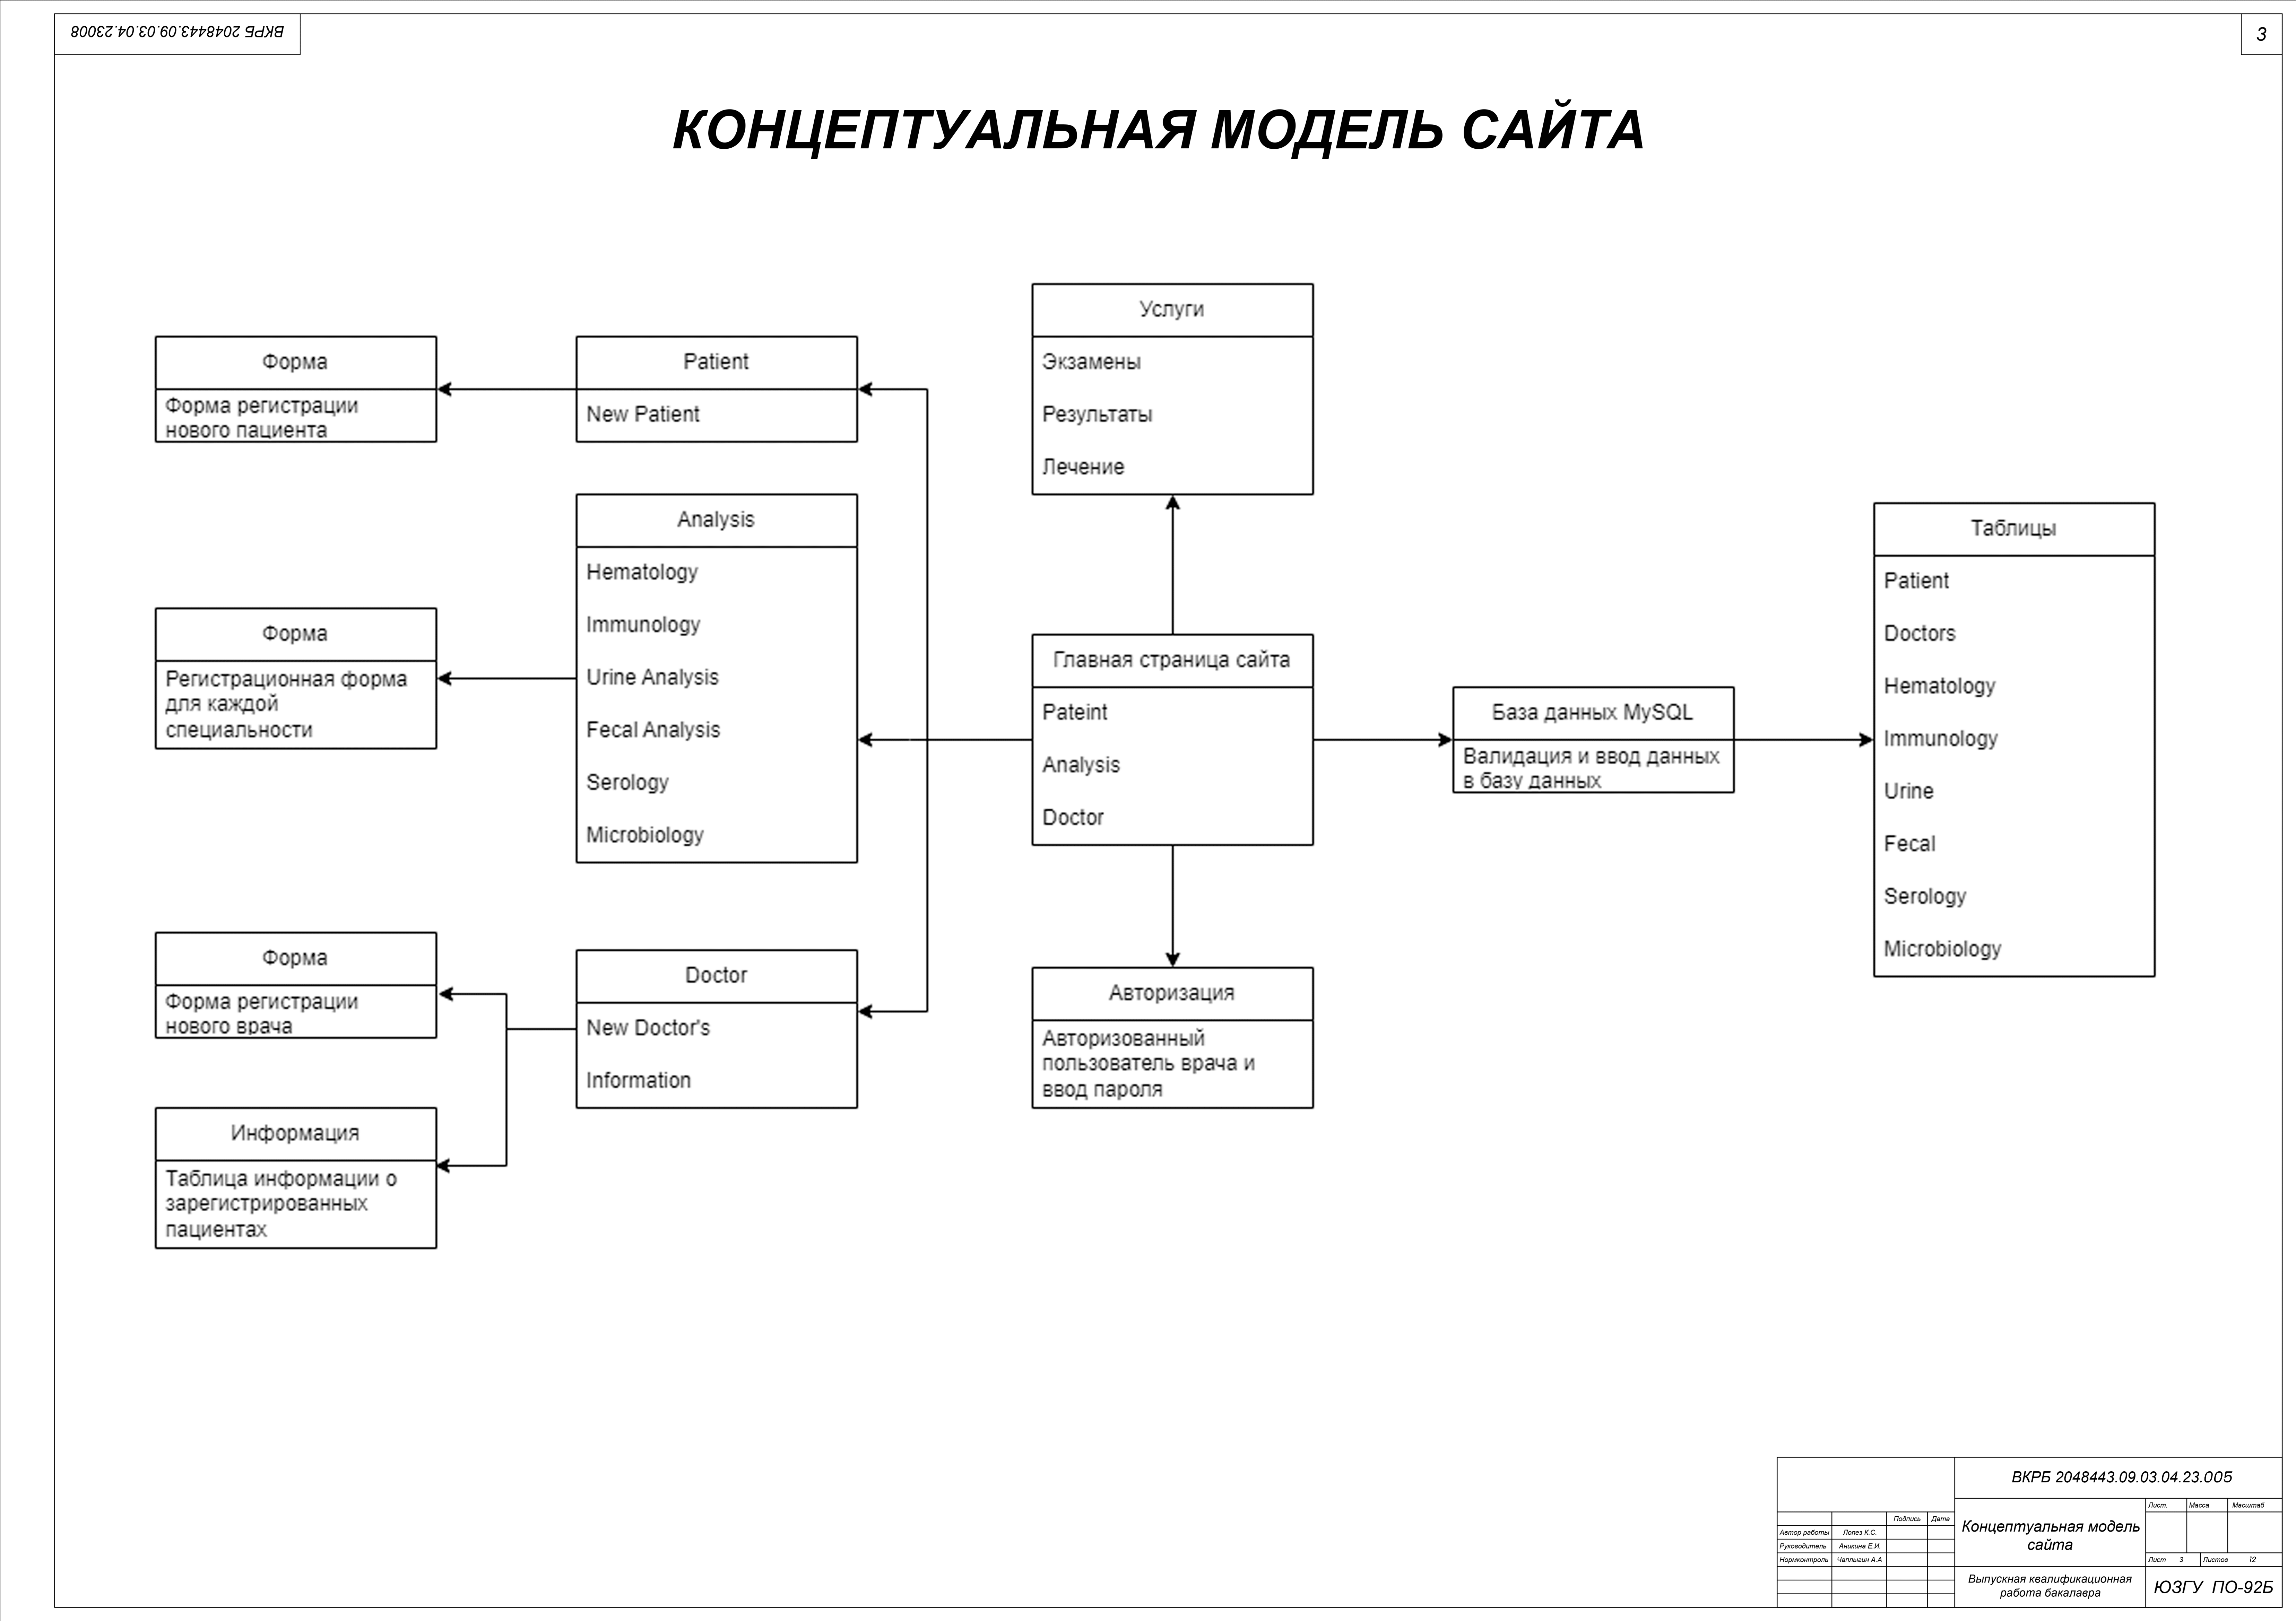
\includegraphics[width=1.3\linewidth]{плакат3.png}
  \end{adjustbox}
  \label{pl3:image}      
\end{figure}

\begin{figure}
	\begin{adjustbox}{addcode={\begin{minipage}{\width}}{\caption{%
						Диаграмма прецедентов
			}\end{minipage}},rotate=90,center}
		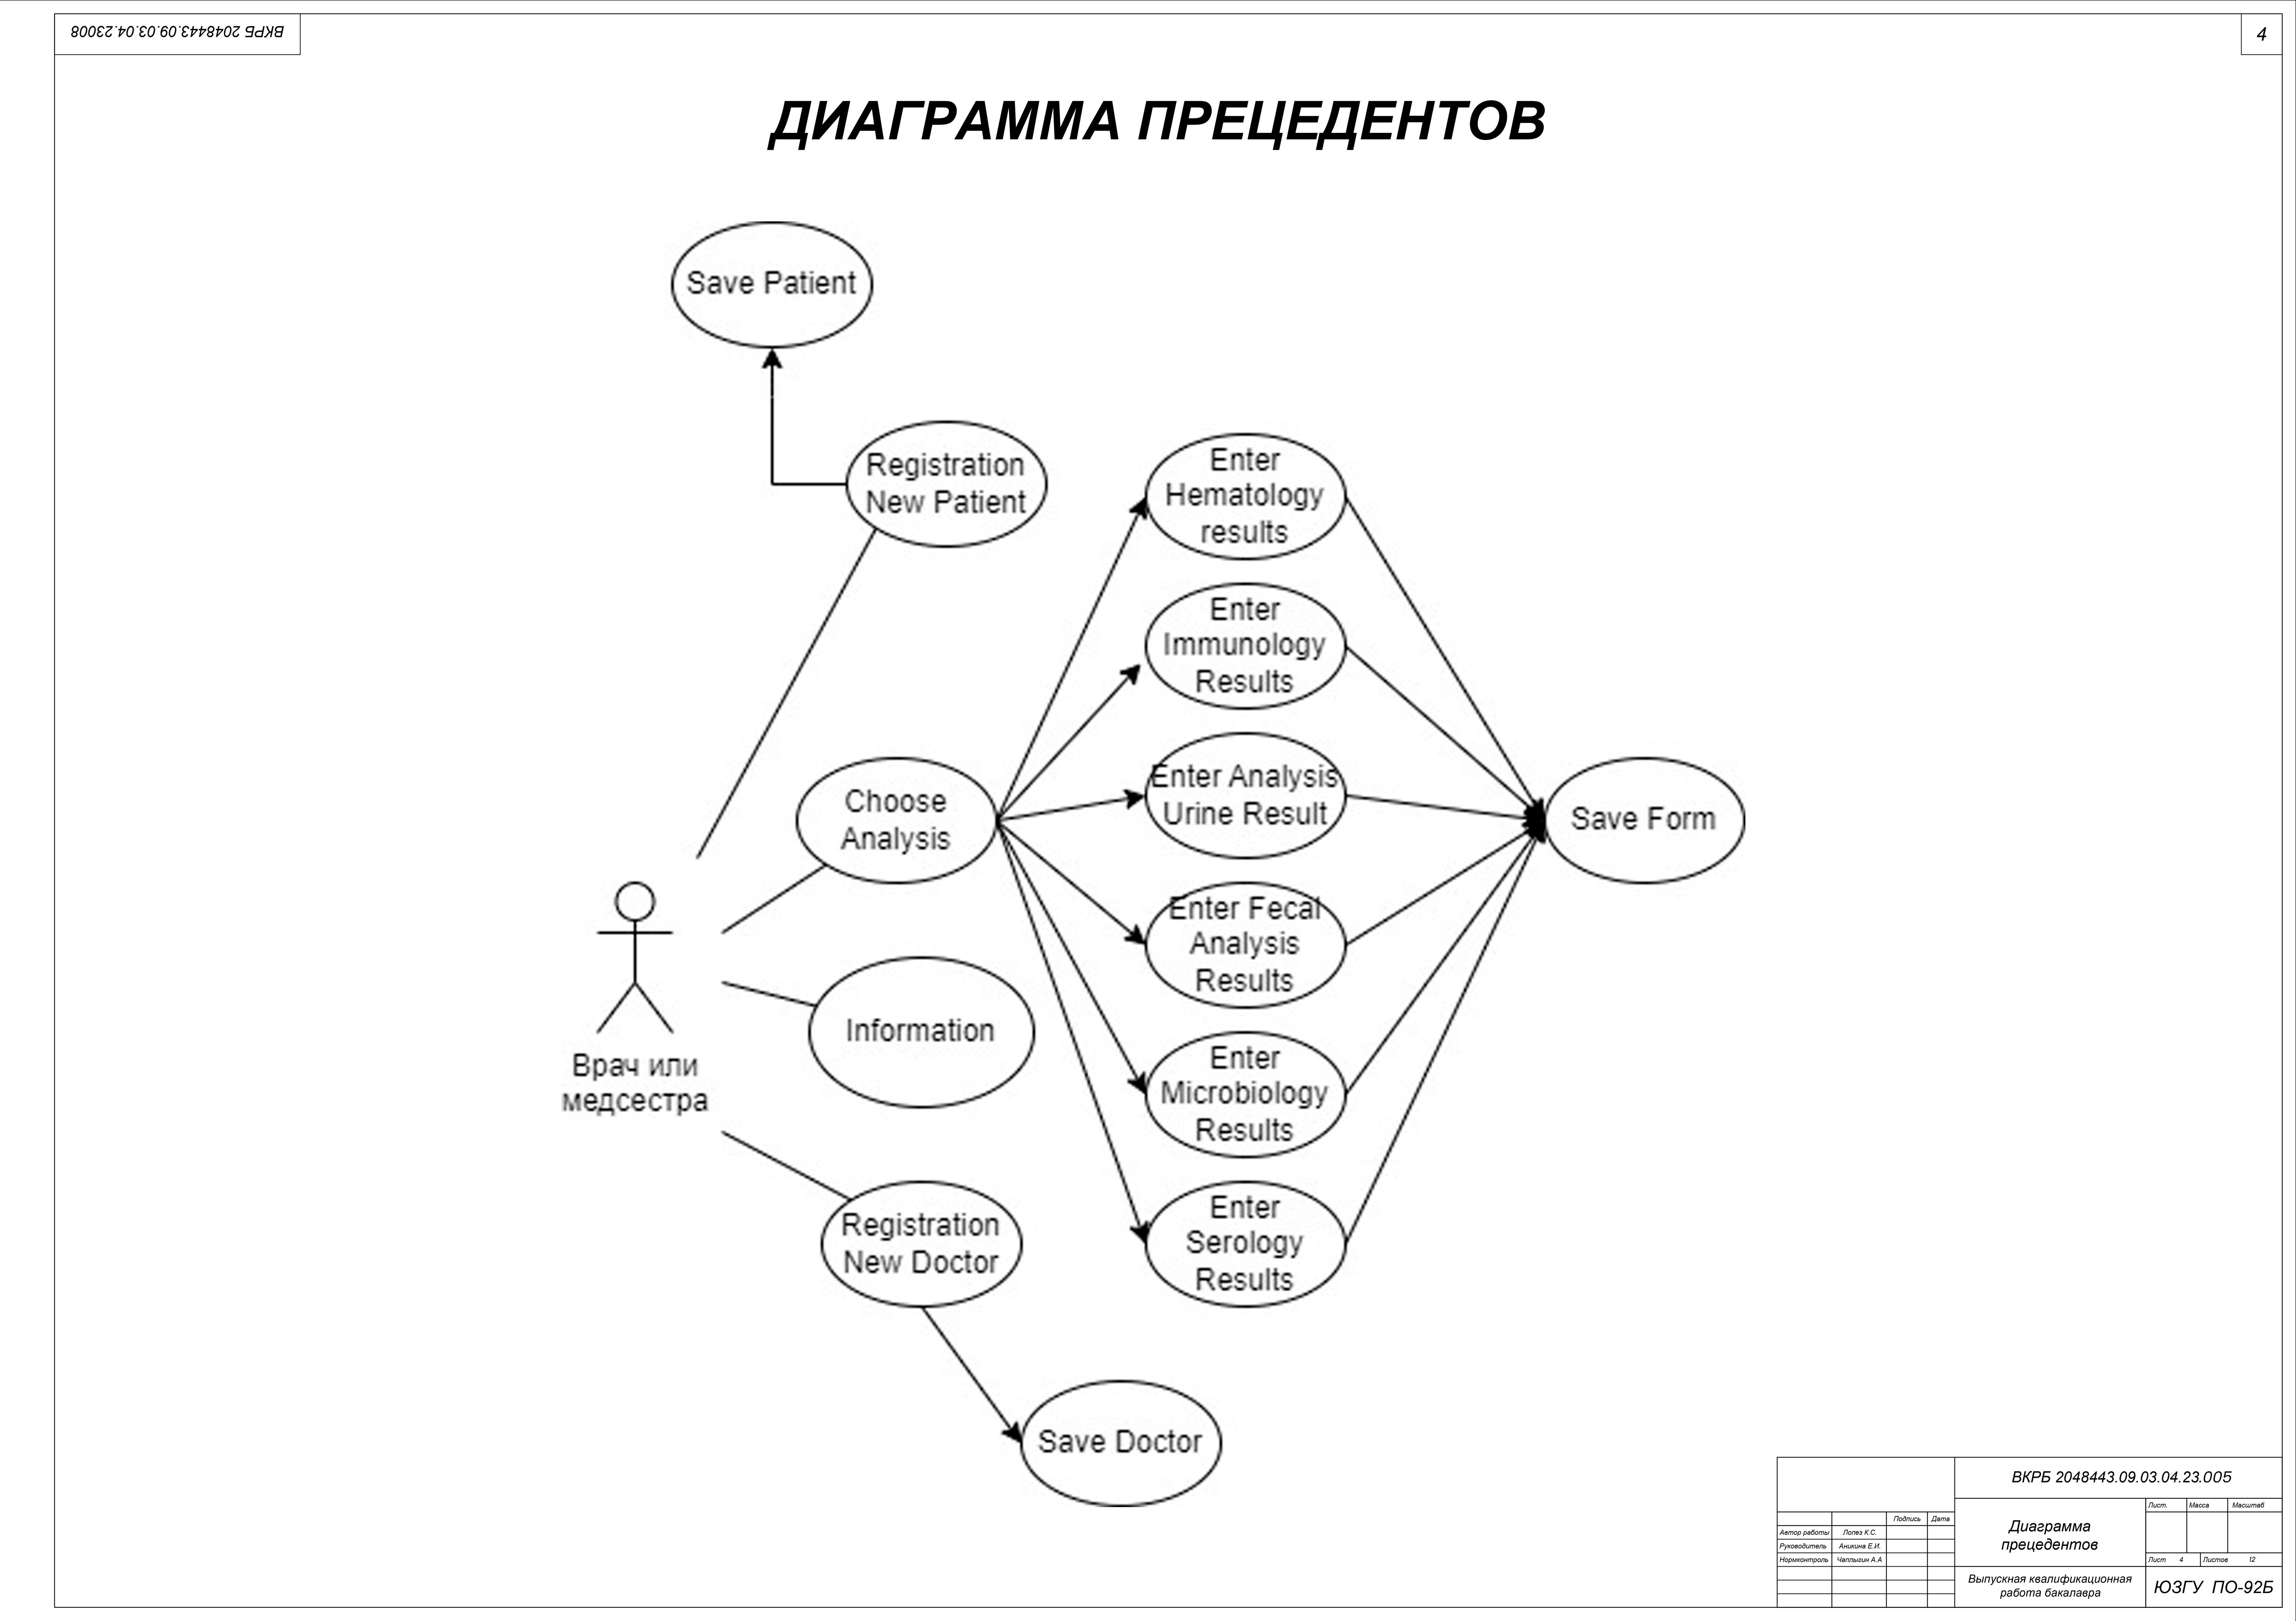
\includegraphics[width=1.3\linewidth]{плакат4.png}
	\end{adjustbox}
	\label{pl4:image}      
\end{figure}

\begin{figure}
	\begin{adjustbox}{addcode={\begin{minipage}{\width}}{\caption{%
						Схема базы данных
			}\end{minipage}},rotate=90,center}
		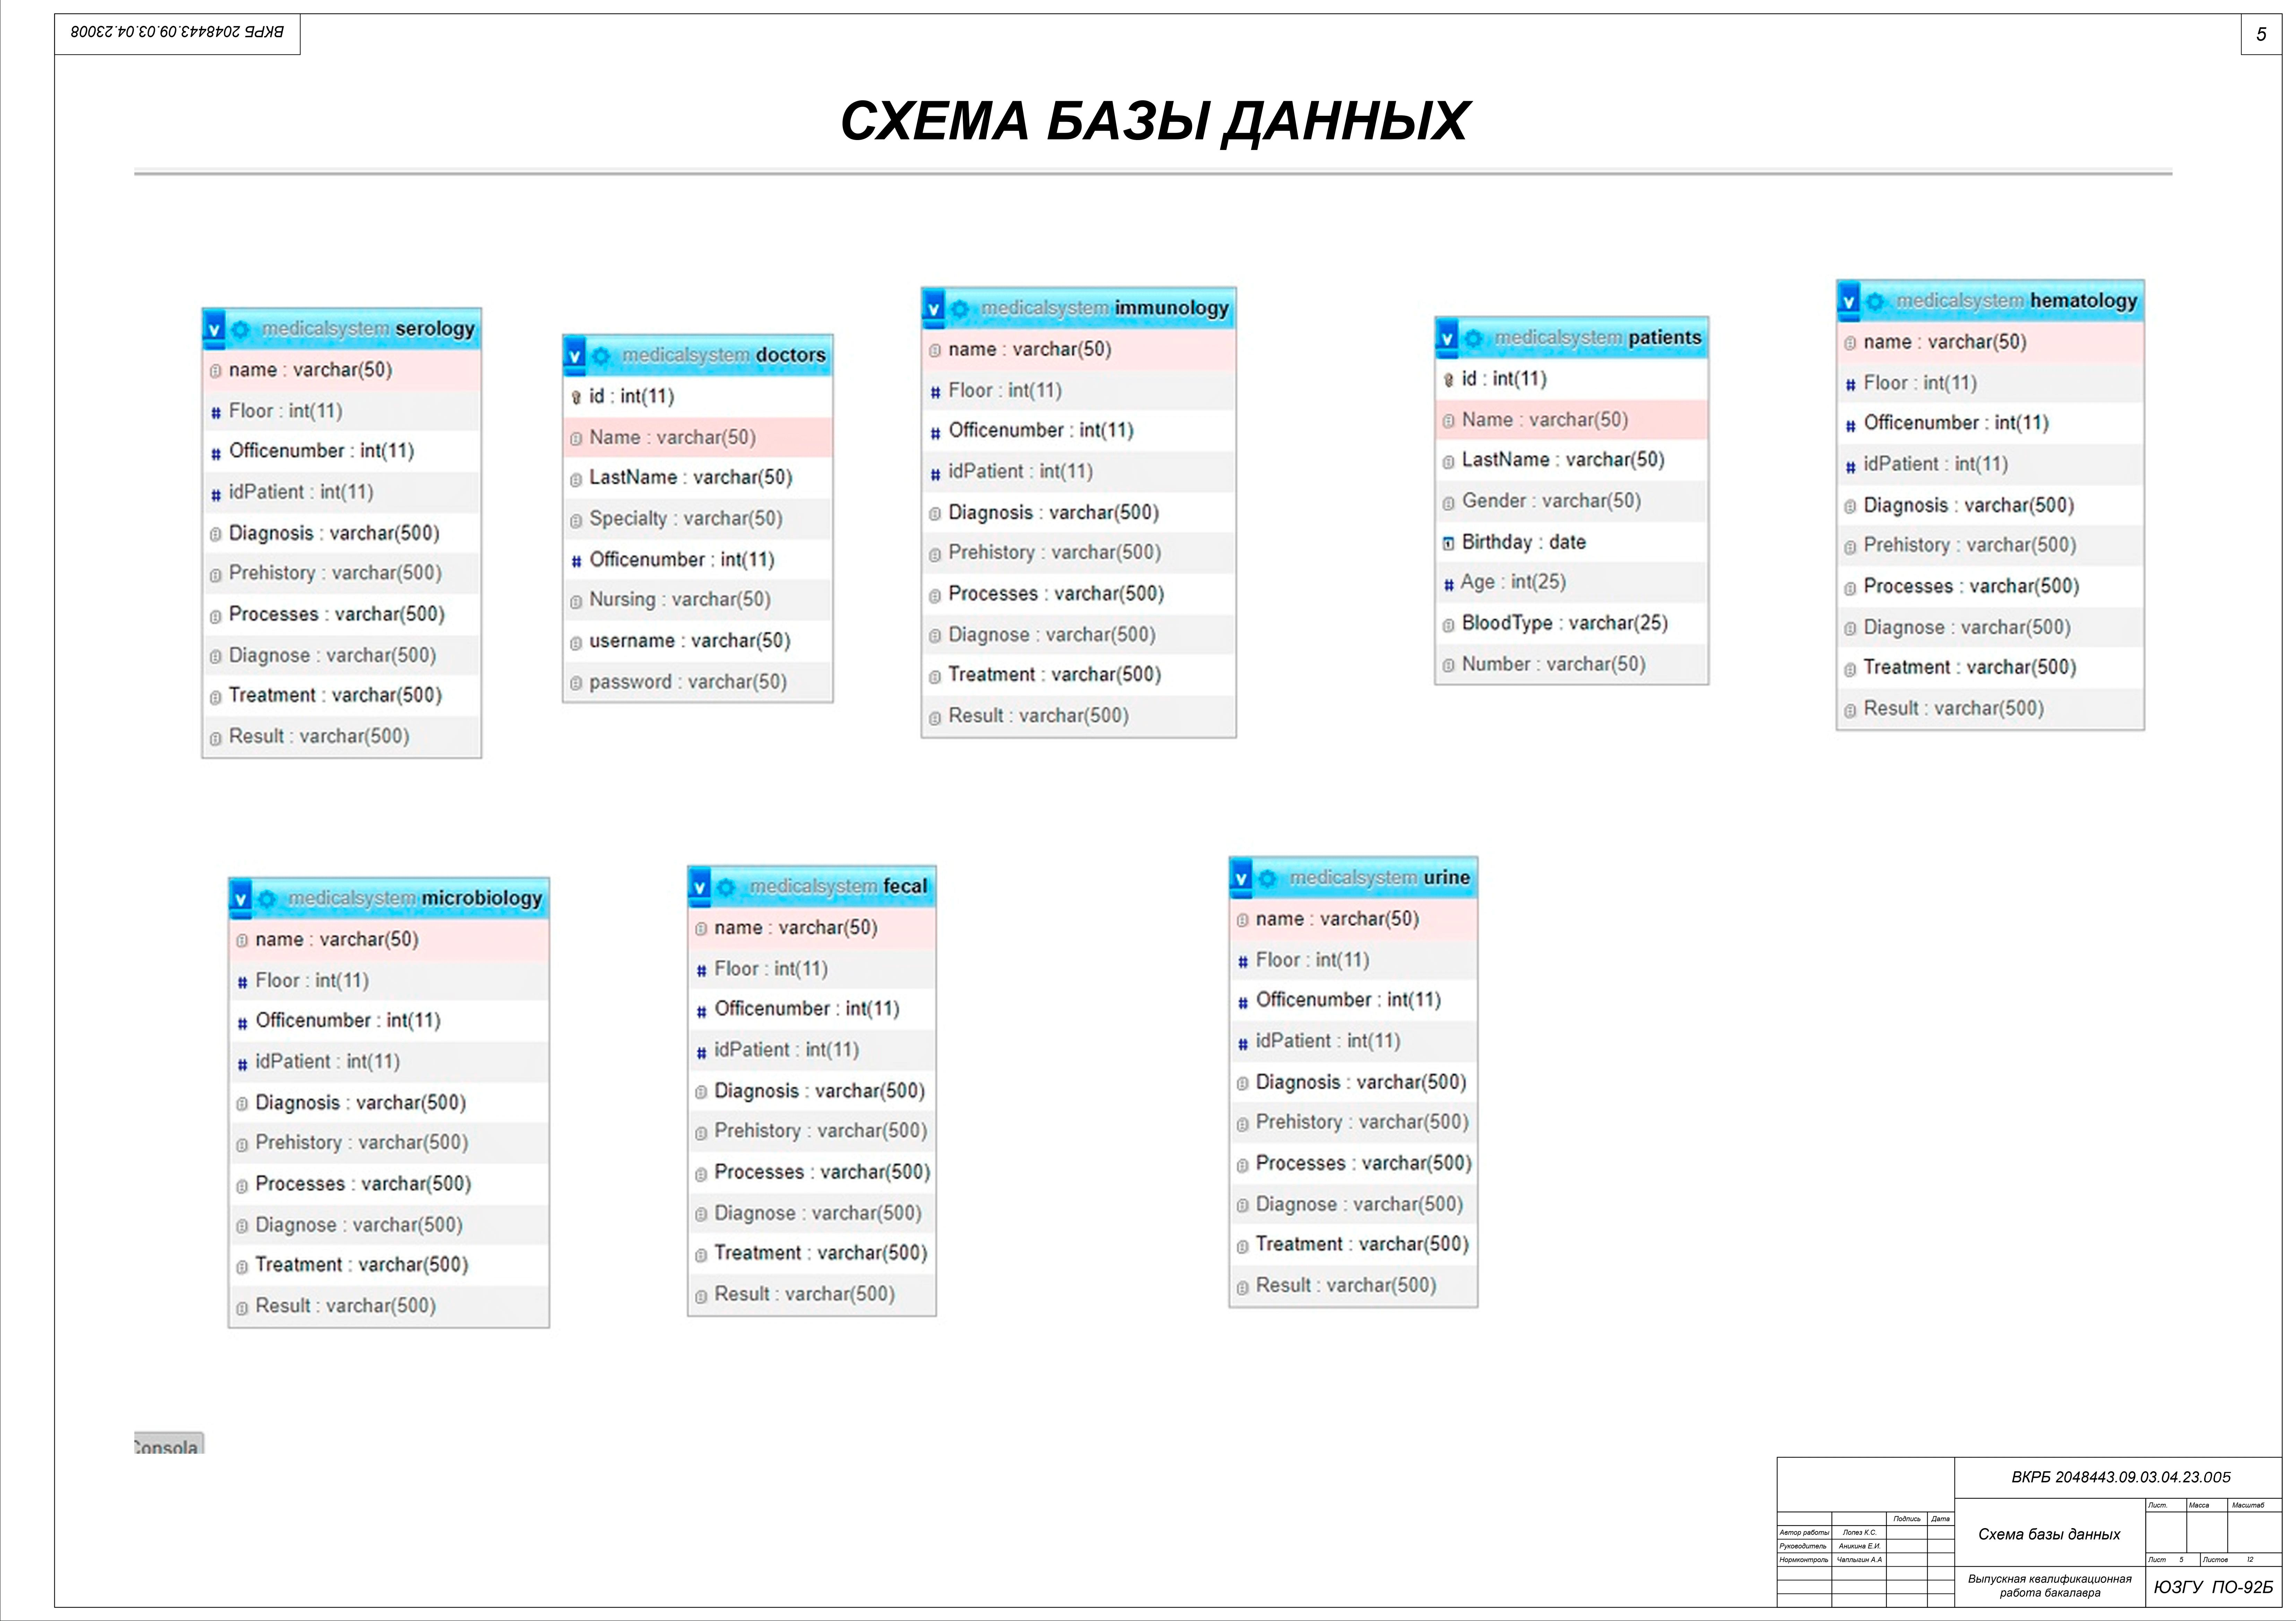
\includegraphics[width=1.3\linewidth]{плакат5.png}
	\end{adjustbox}
	\label{pl5:image}      
\end{figure}

\begin{figure}
	\begin{adjustbox}{addcode={\begin{minipage}{\width}}{\caption{%
						Диаграмма развертывания
			}\end{minipage}},rotate=90,center}
		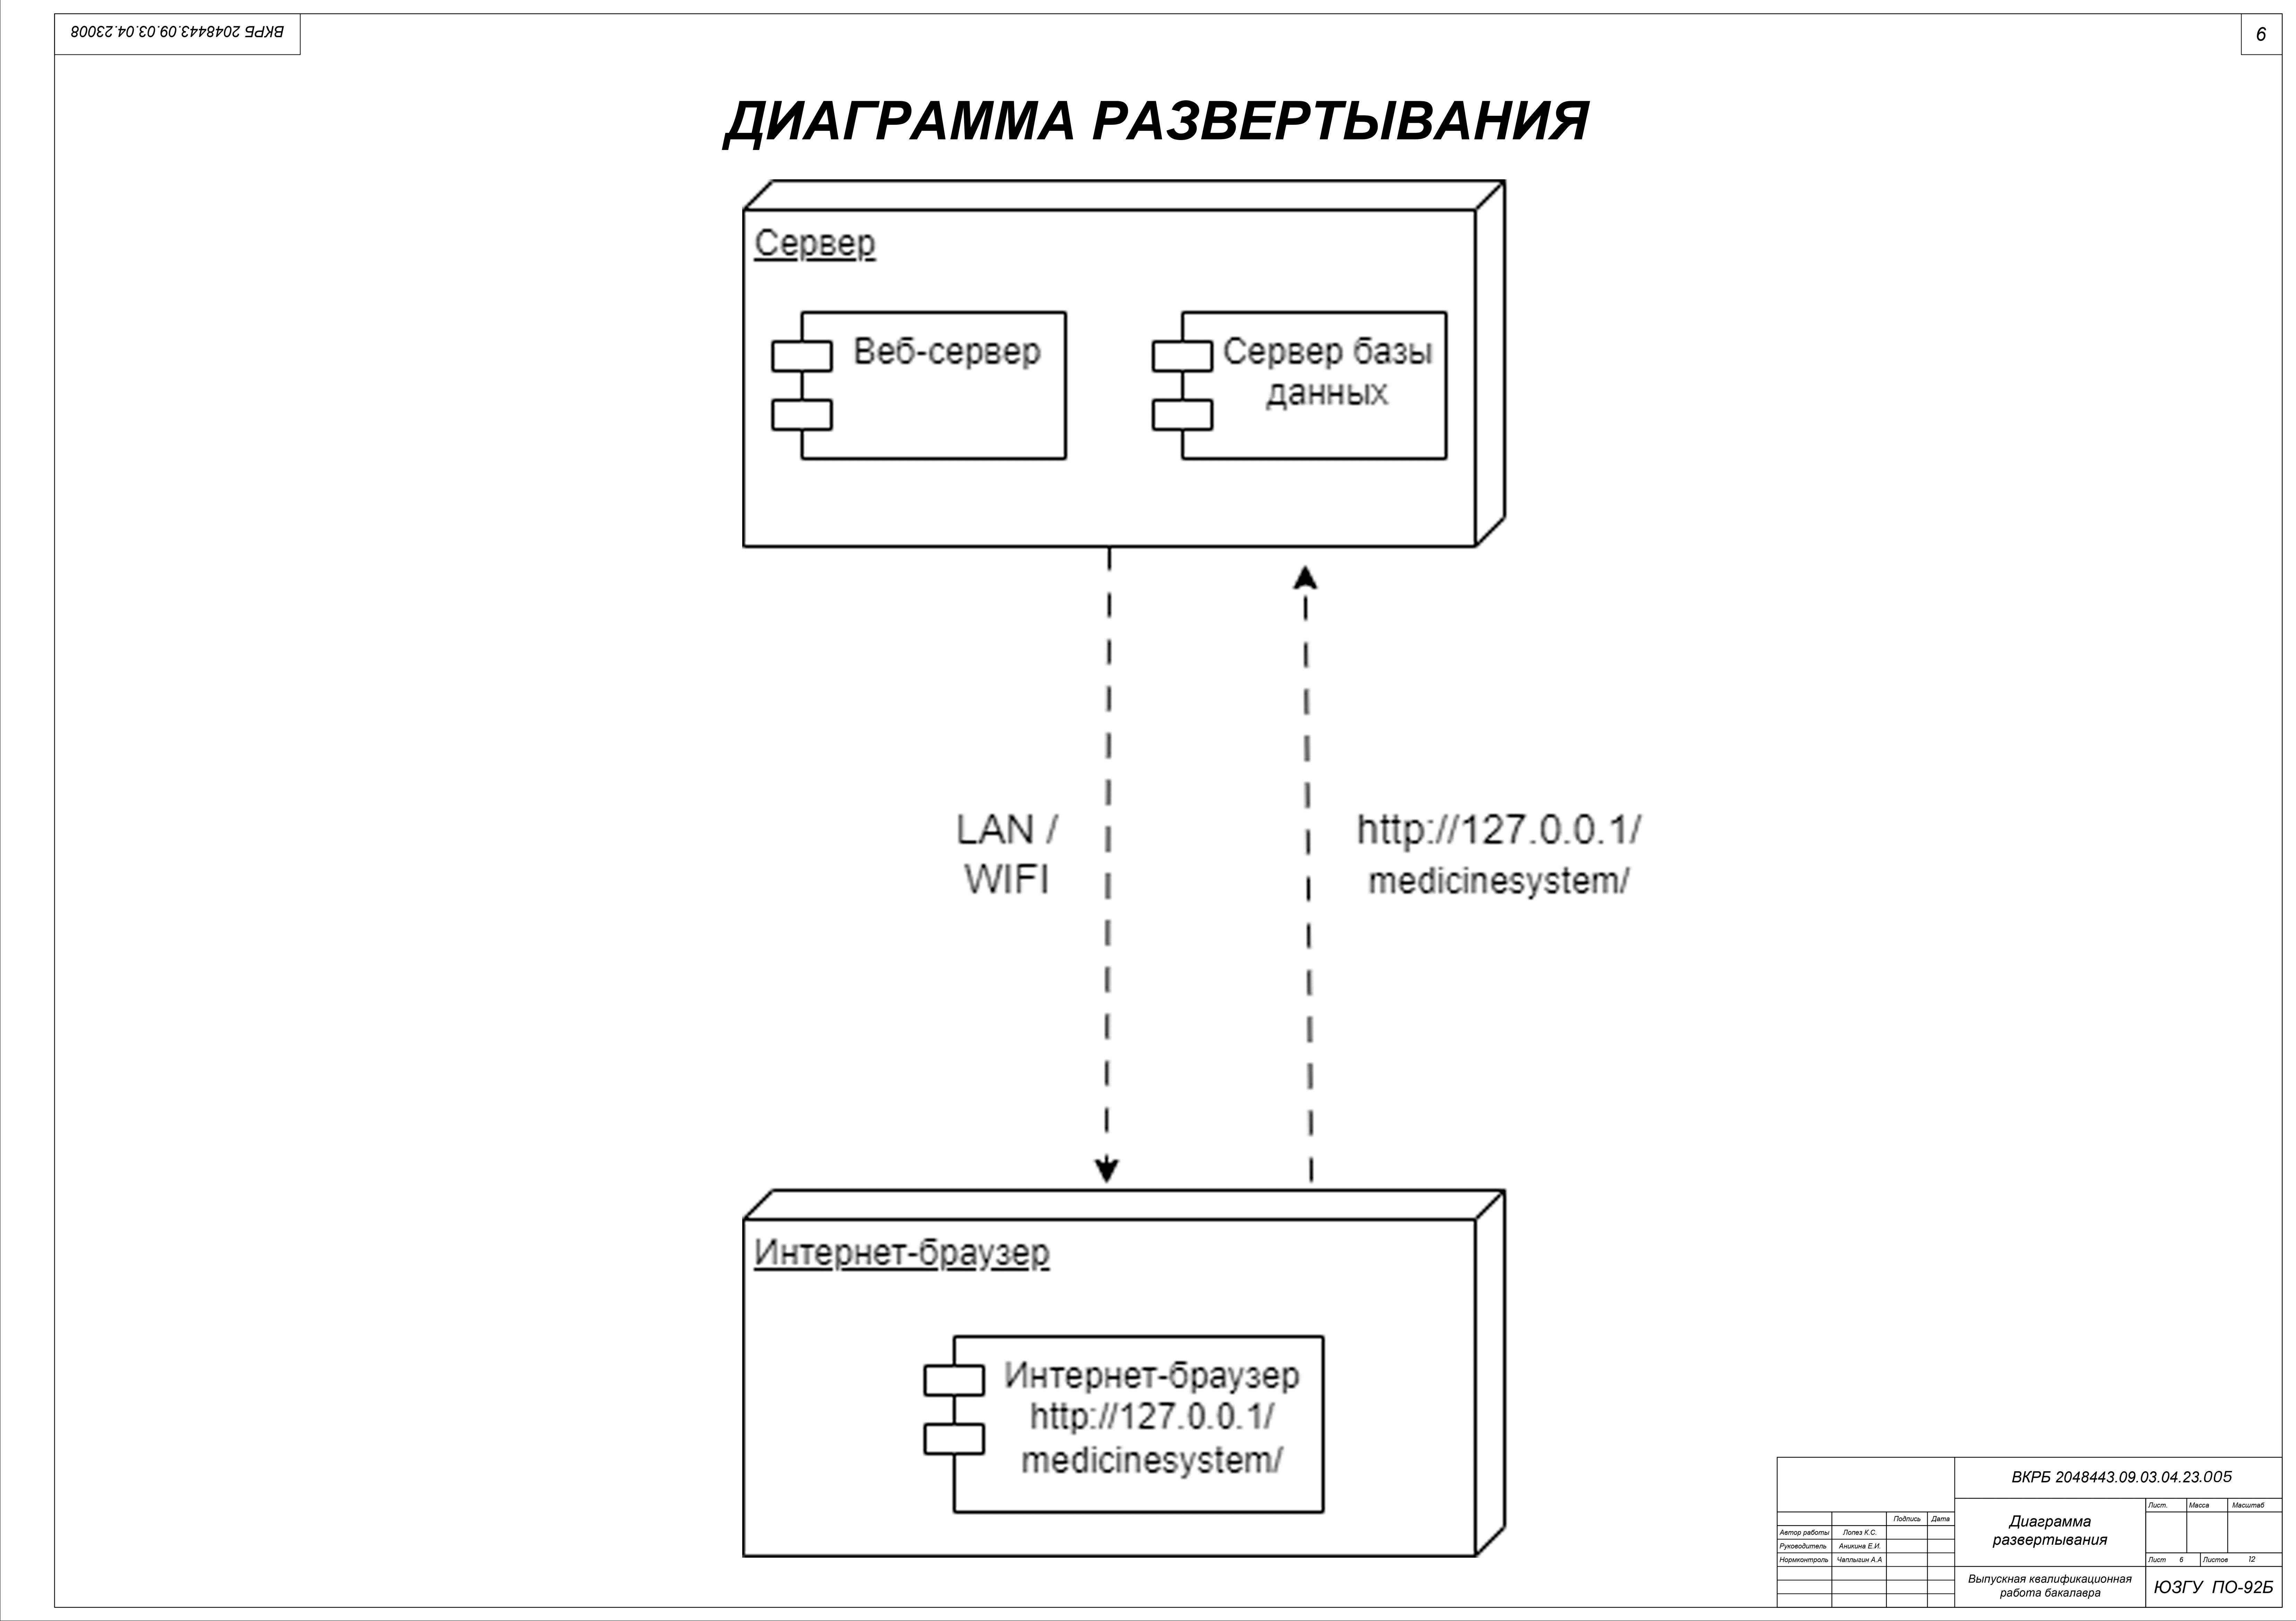
\includegraphics[width=1.3\linewidth]{плакат6.png}
	\end{adjustbox}
	\label{pl6:image}      
\end{figure}

\begin{figure}
	\begin{adjustbox}{addcode={\begin{minipage}{\width}}{\caption{%
						Диаграмма классов
			}\end{minipage}},rotate=90,center}
		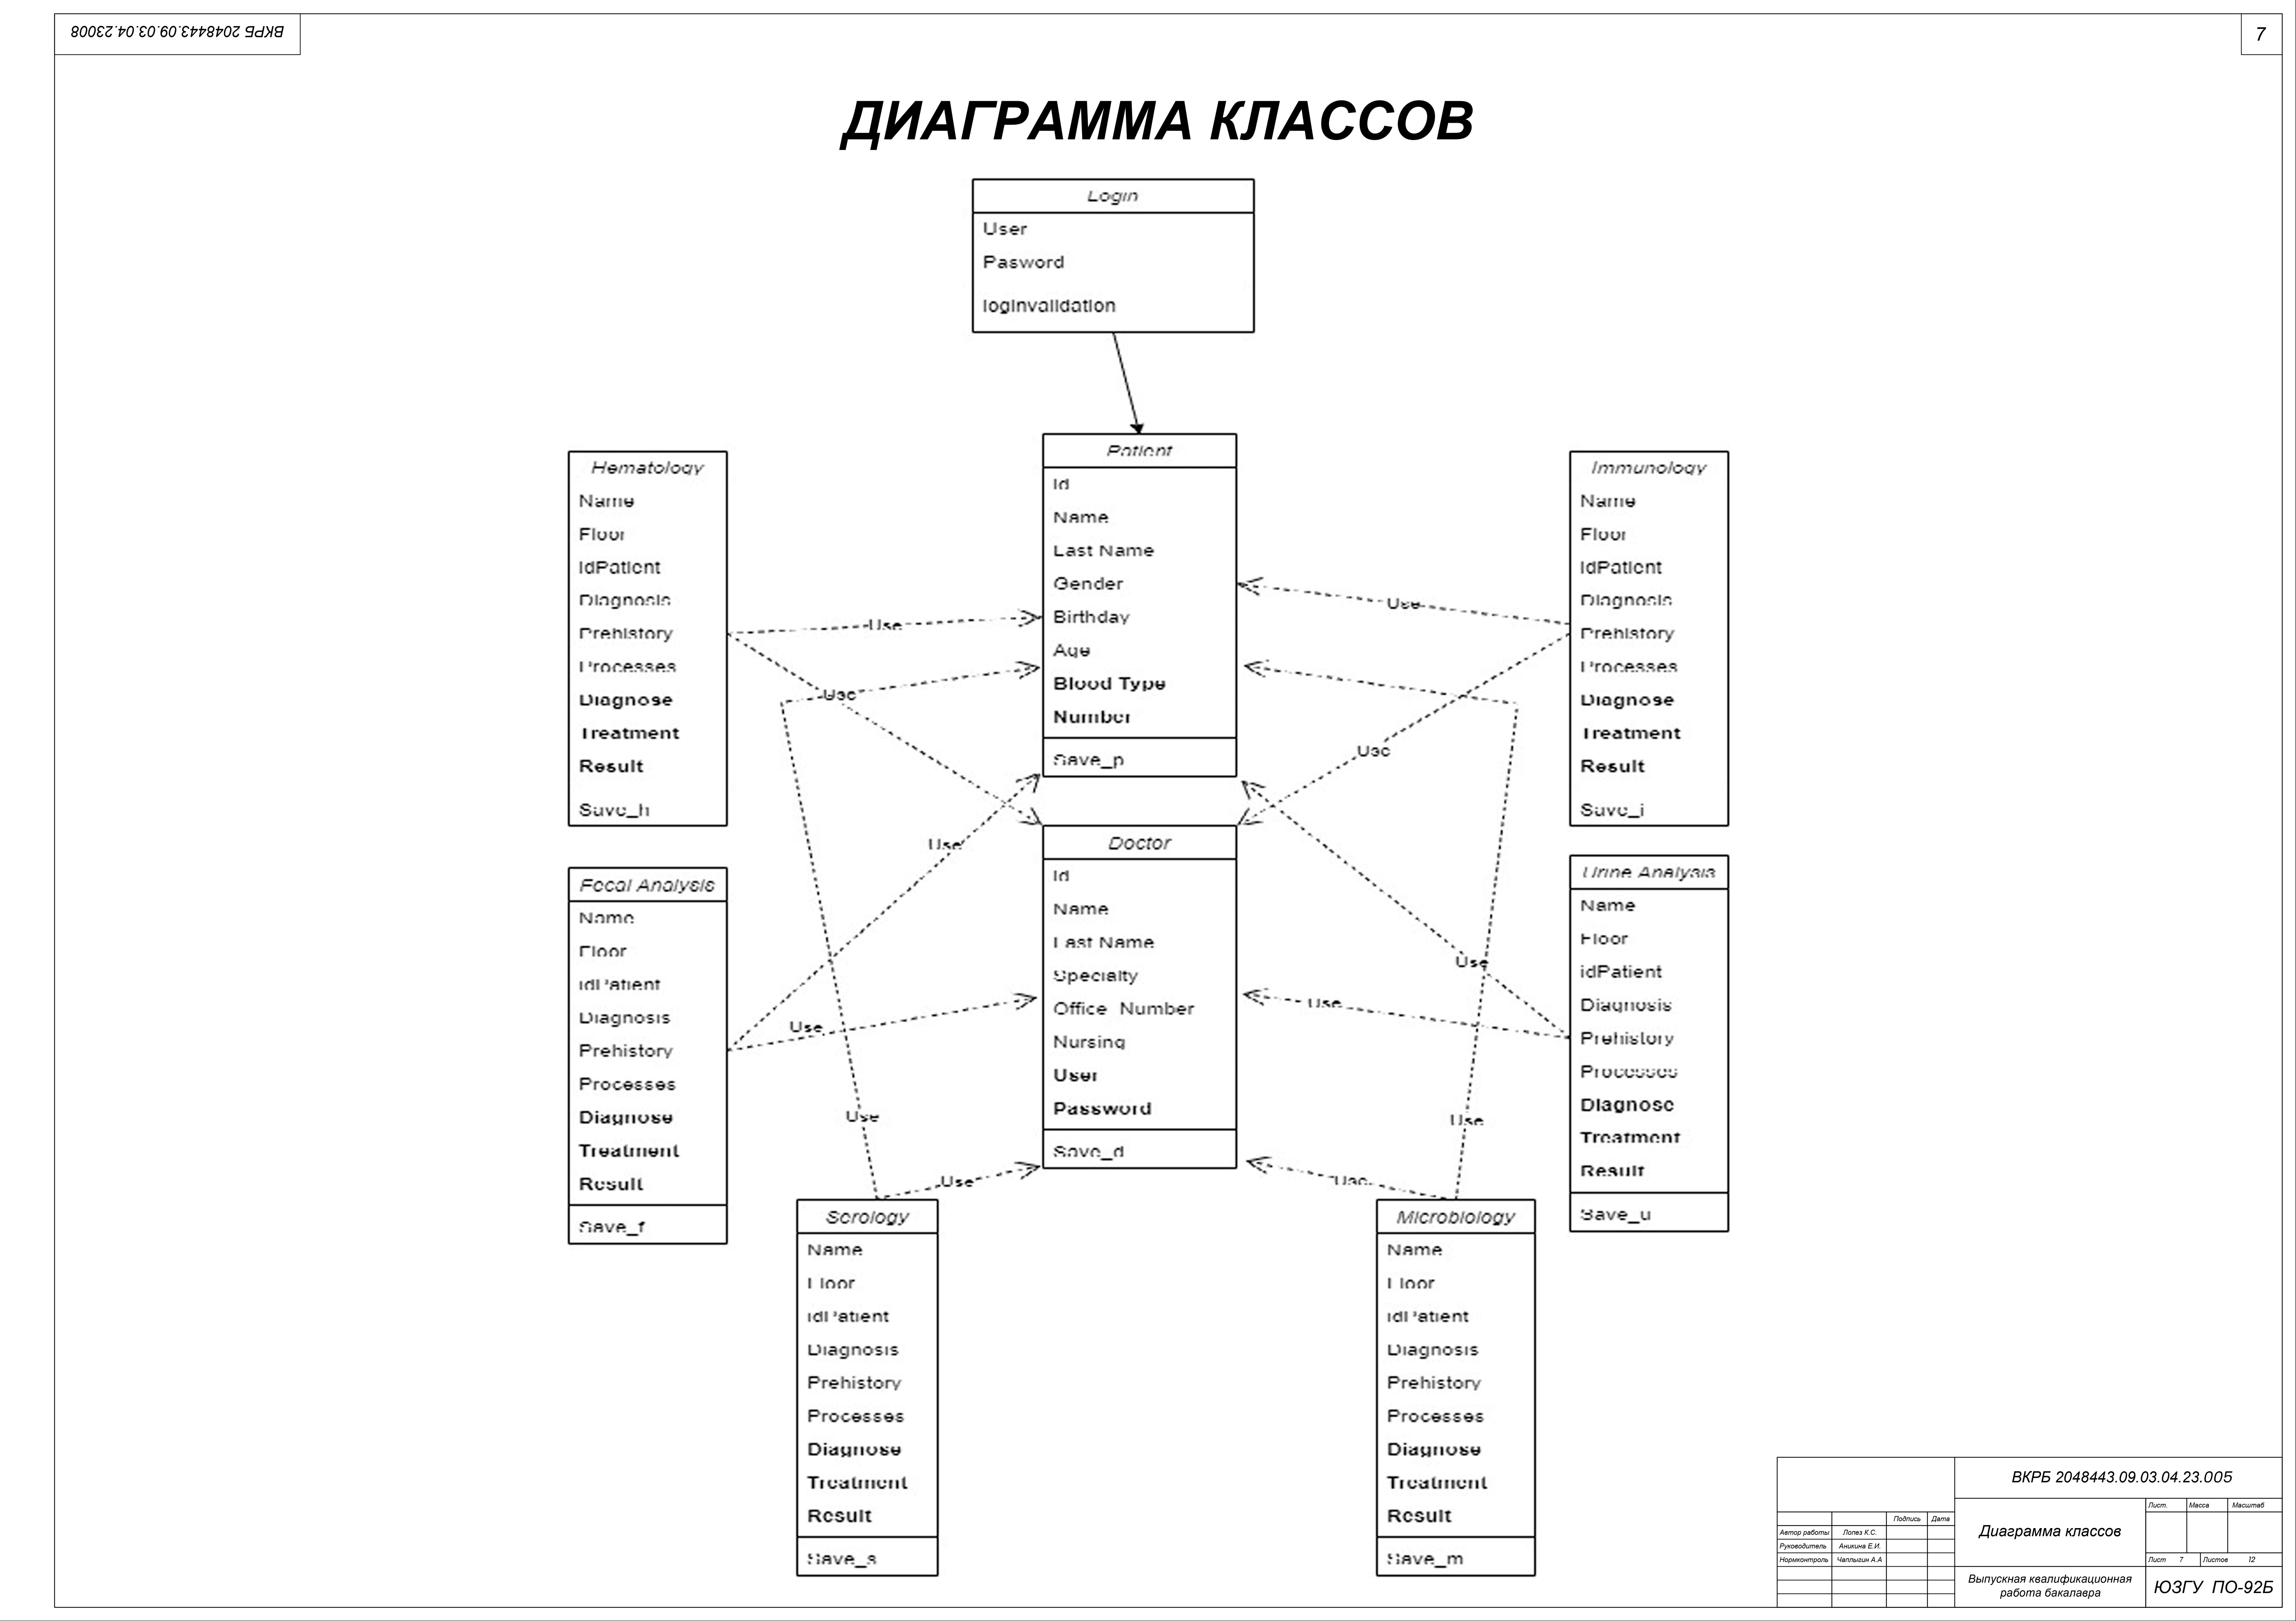
\includegraphics[width=1.3\linewidth]{плакат7.png}
	\end{adjustbox}
	\label{pl7:image}      
\end{figure}

\begin{figure}
	\begin{adjustbox}{addcode={\begin{minipage}{\width}}{\caption{%
						Дизайн интерфейса. Веб-страница авторизации
			}\end{minipage}},rotate=90,center}
		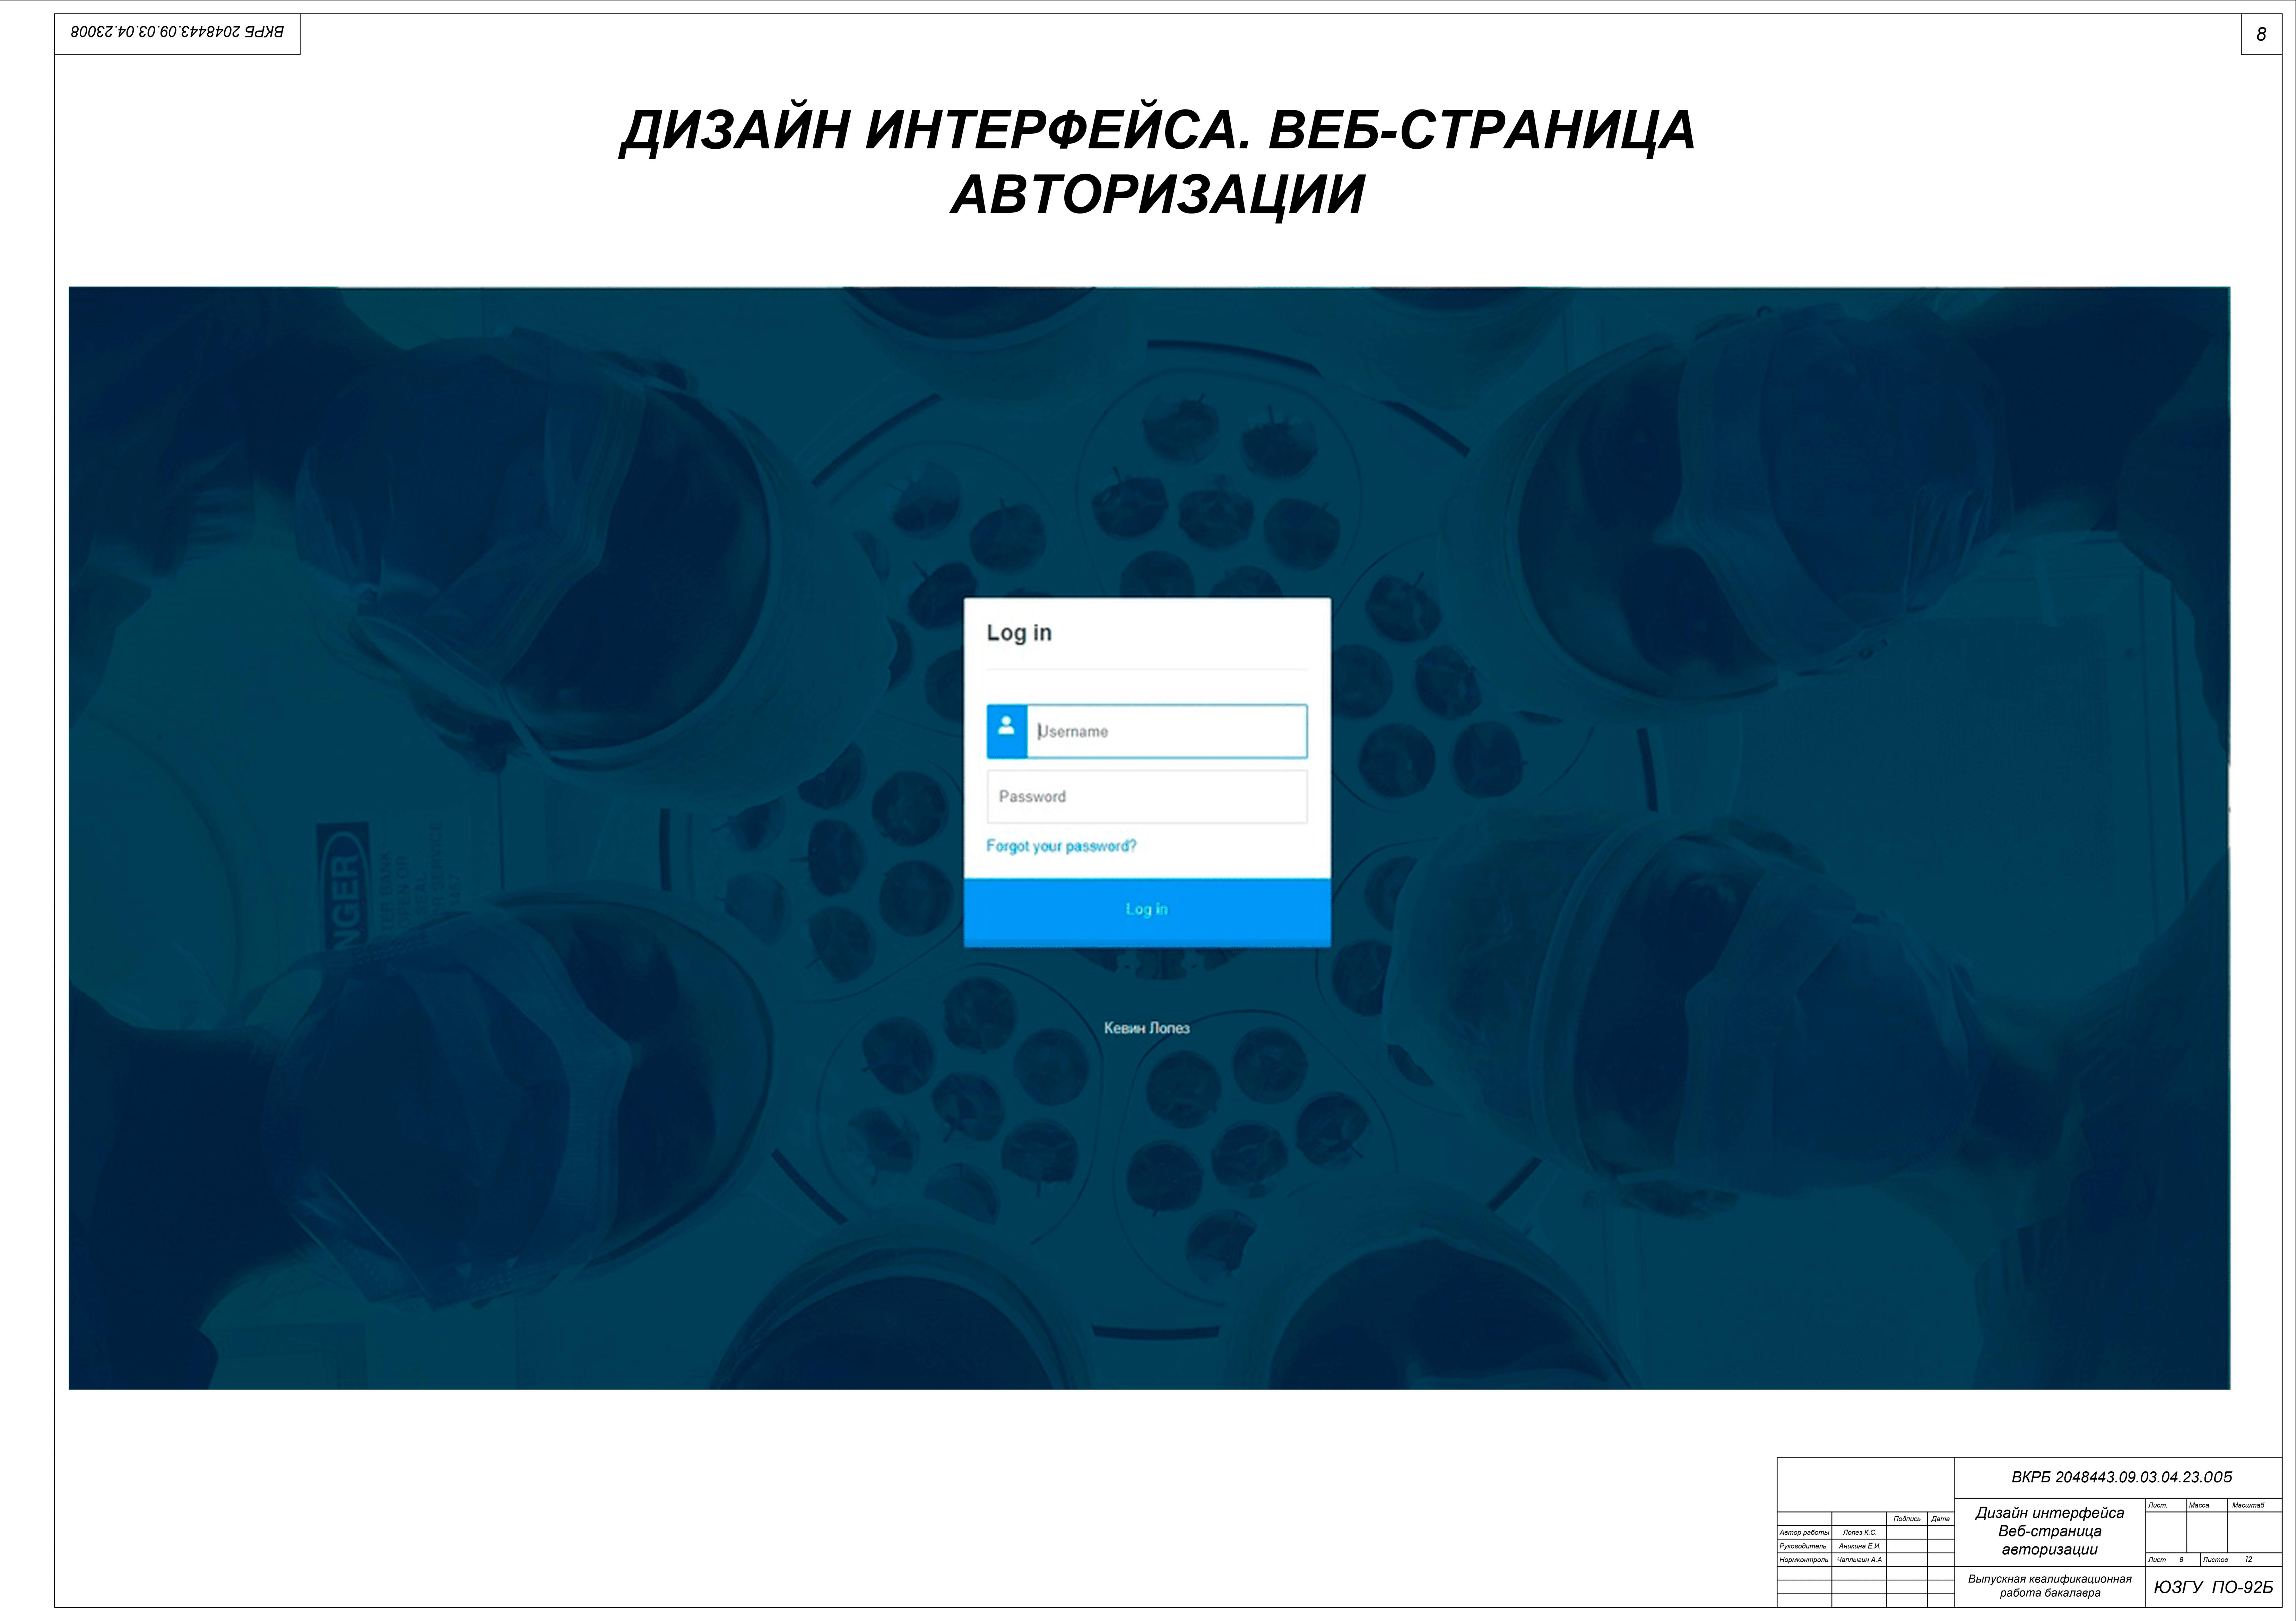
\includegraphics[width=1.3\linewidth]{плакат8.png}
	\end{adjustbox}
	\label{pl8:image}      
\end{figure}

\begin{figure}
	\begin{adjustbox}{addcode={\begin{minipage}{\width}}{\caption{%
						Дизайн интерфейса. Веб-страница регистрации пациента
			}\end{minipage}},rotate=90,center}
		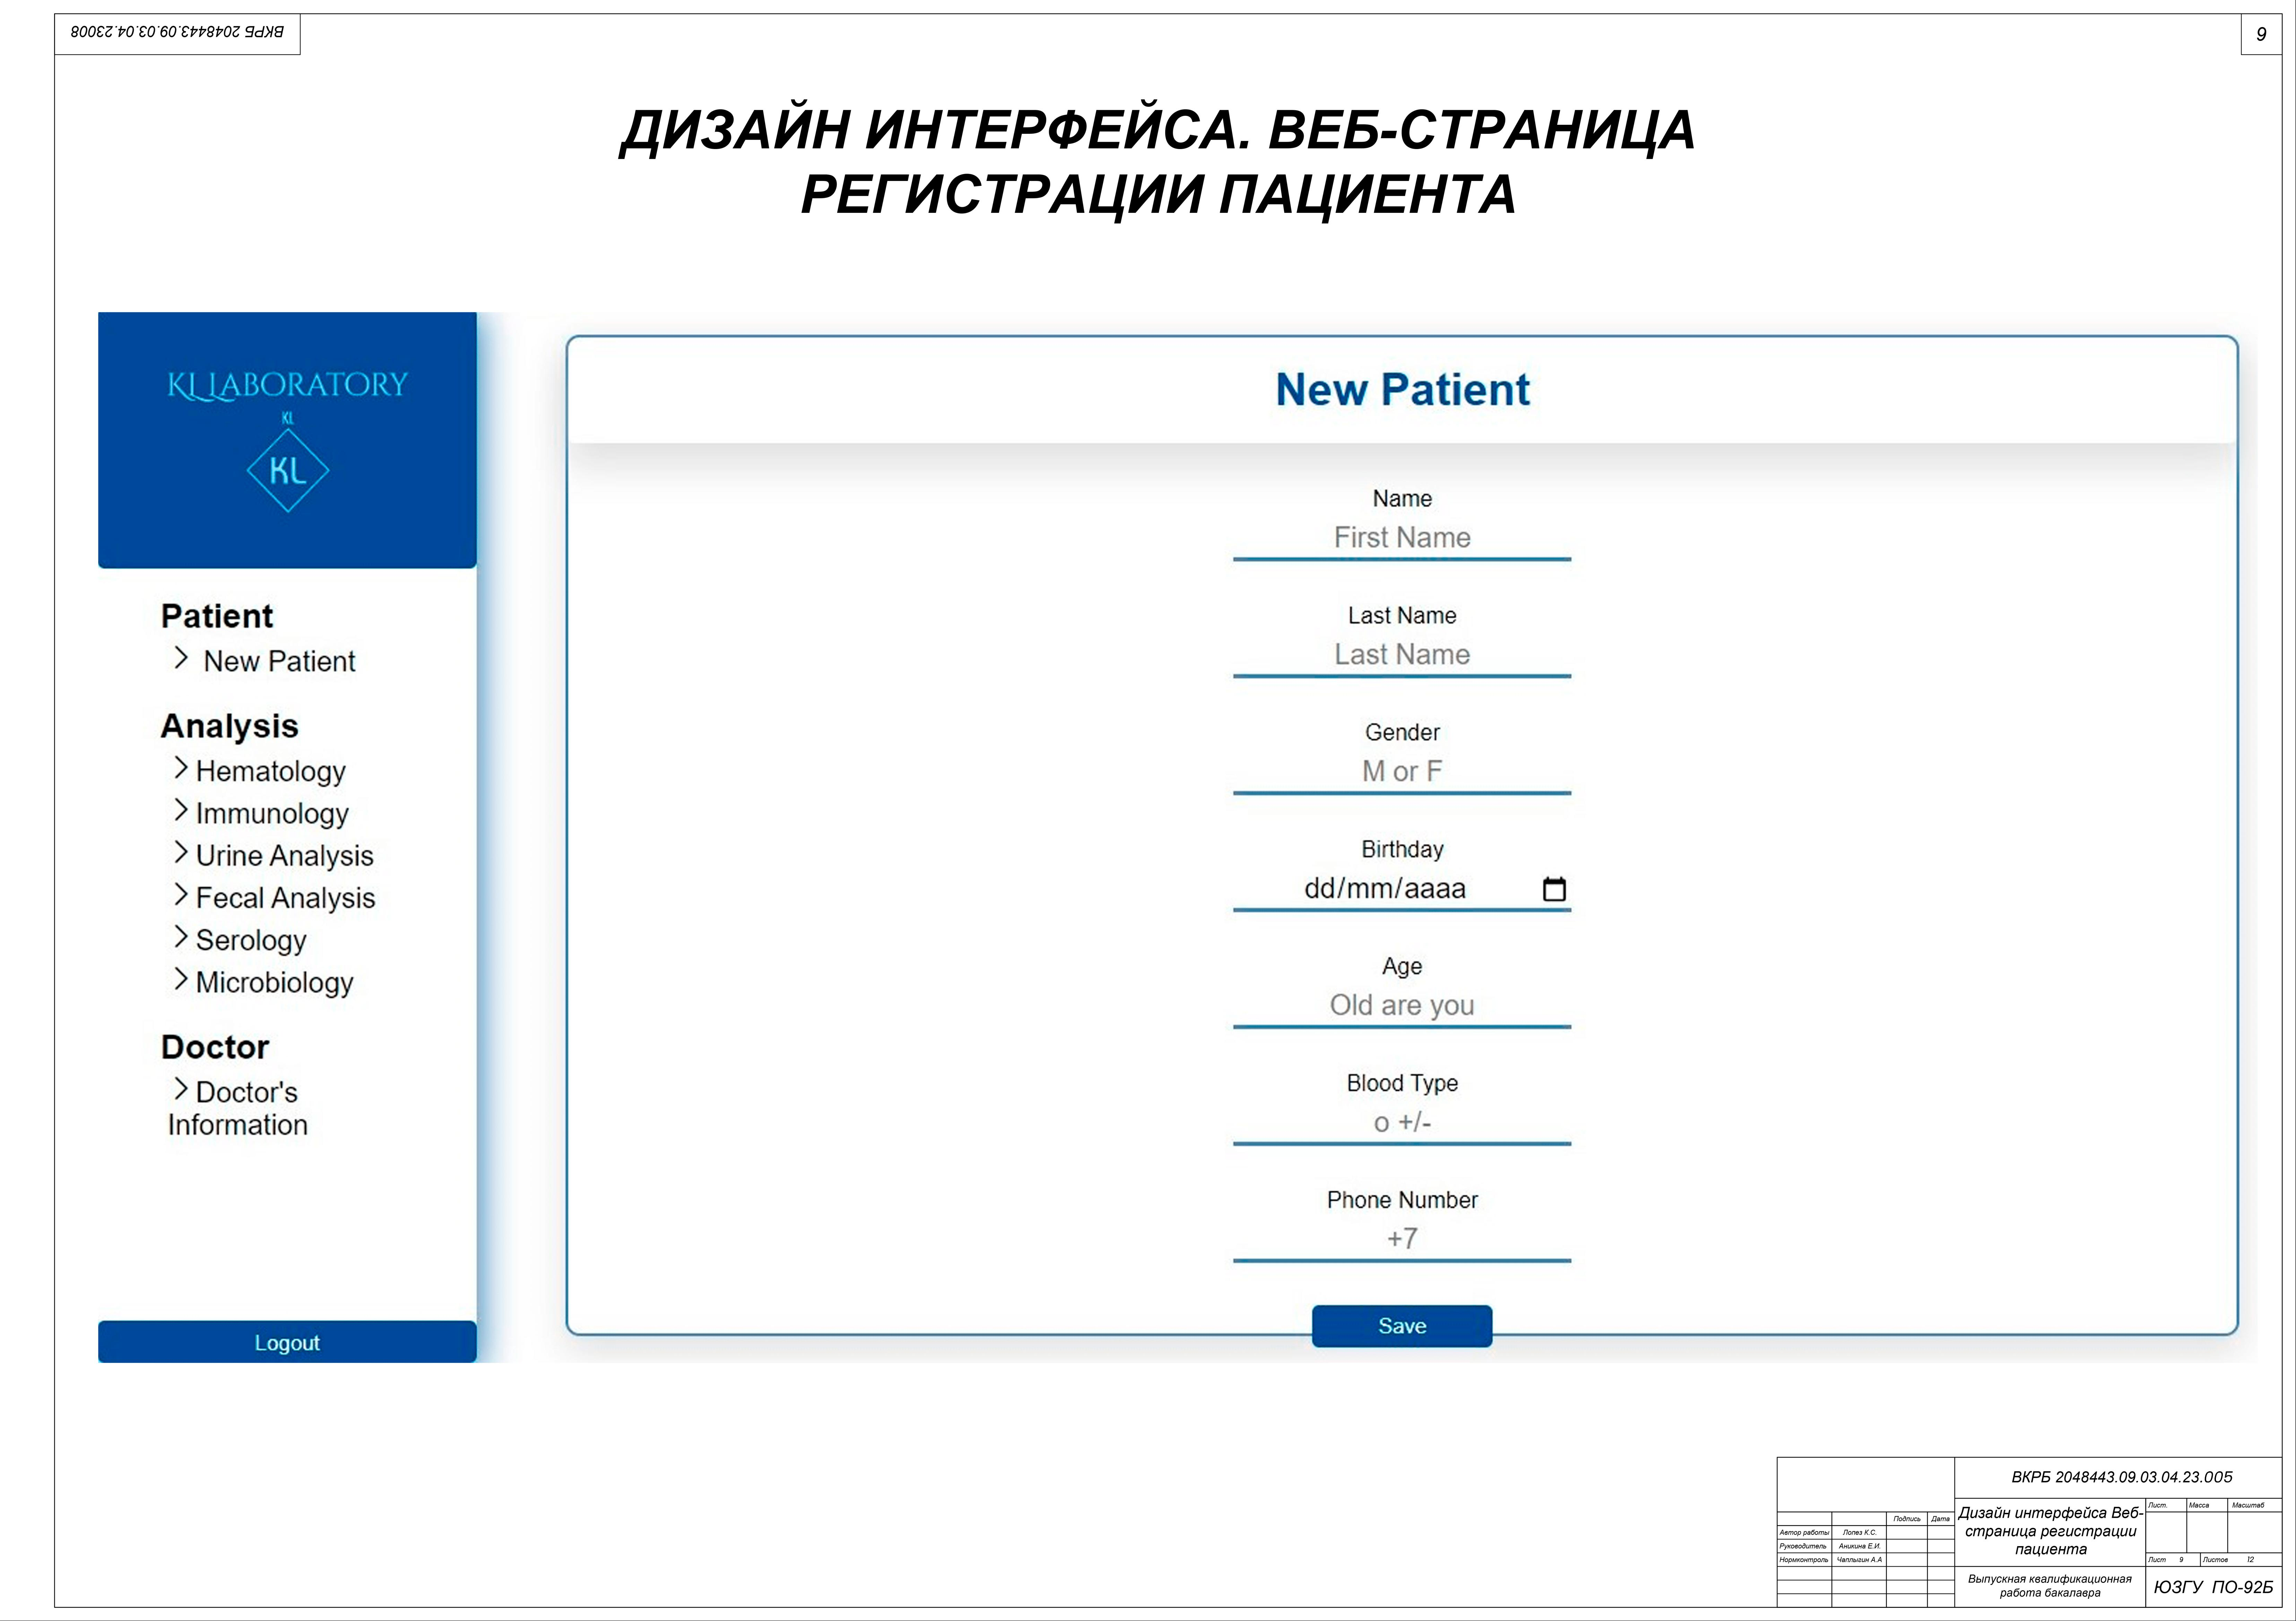
\includegraphics[width=1.3\linewidth]{плакат9.png}
	\end{adjustbox}
	\label{pl9:image}      
\end{figure}

\begin{figure}
	\begin{adjustbox}{addcode={\begin{minipage}{\width}}{\caption{%
						Дизайн интерфейса. Веб-страница регистрации врача
			}\end{minipage}},rotate=90,center}
		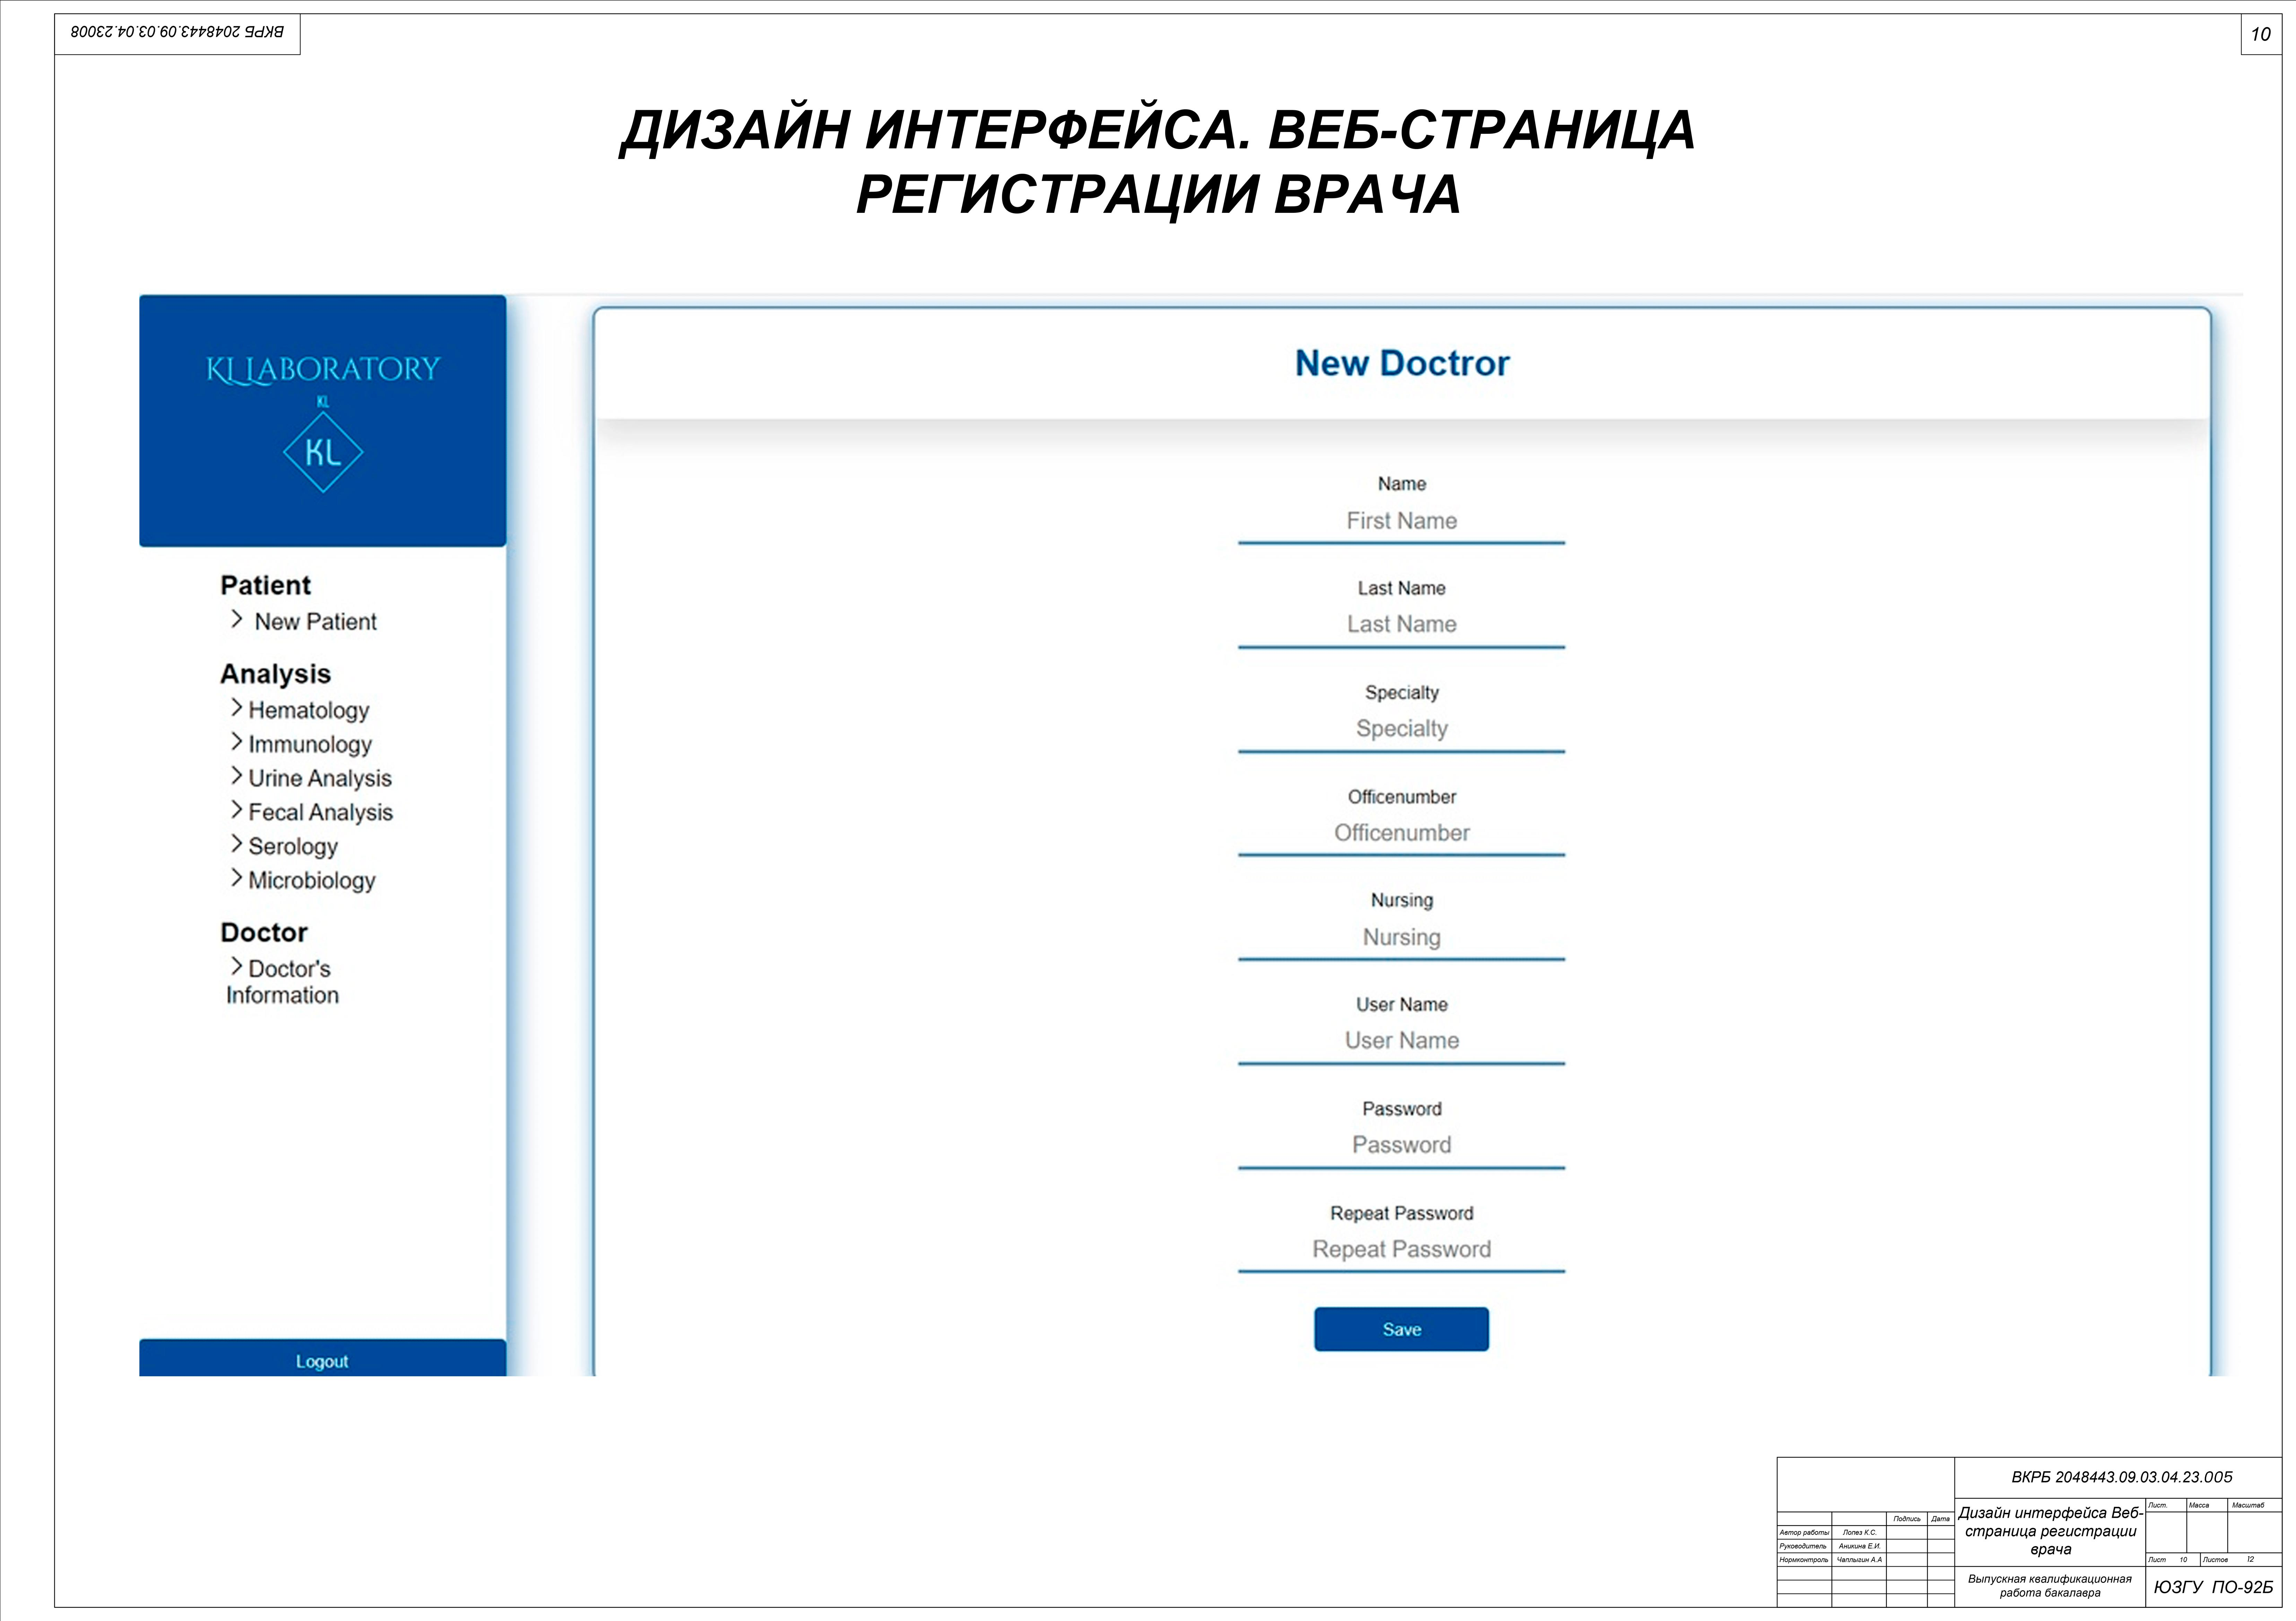
\includegraphics[width=1.3\linewidth]{плакат10.png}
	\end{adjustbox}
	\label{pl10:image}      
\end{figure}

\begin{figure}
	\begin{adjustbox}{addcode={\begin{minipage}{\width}}{\caption{%
						Дизайн интерфейса. Веб-страница для ввода результатов анализа крови
			}\end{minipage}},rotate=90,center}
		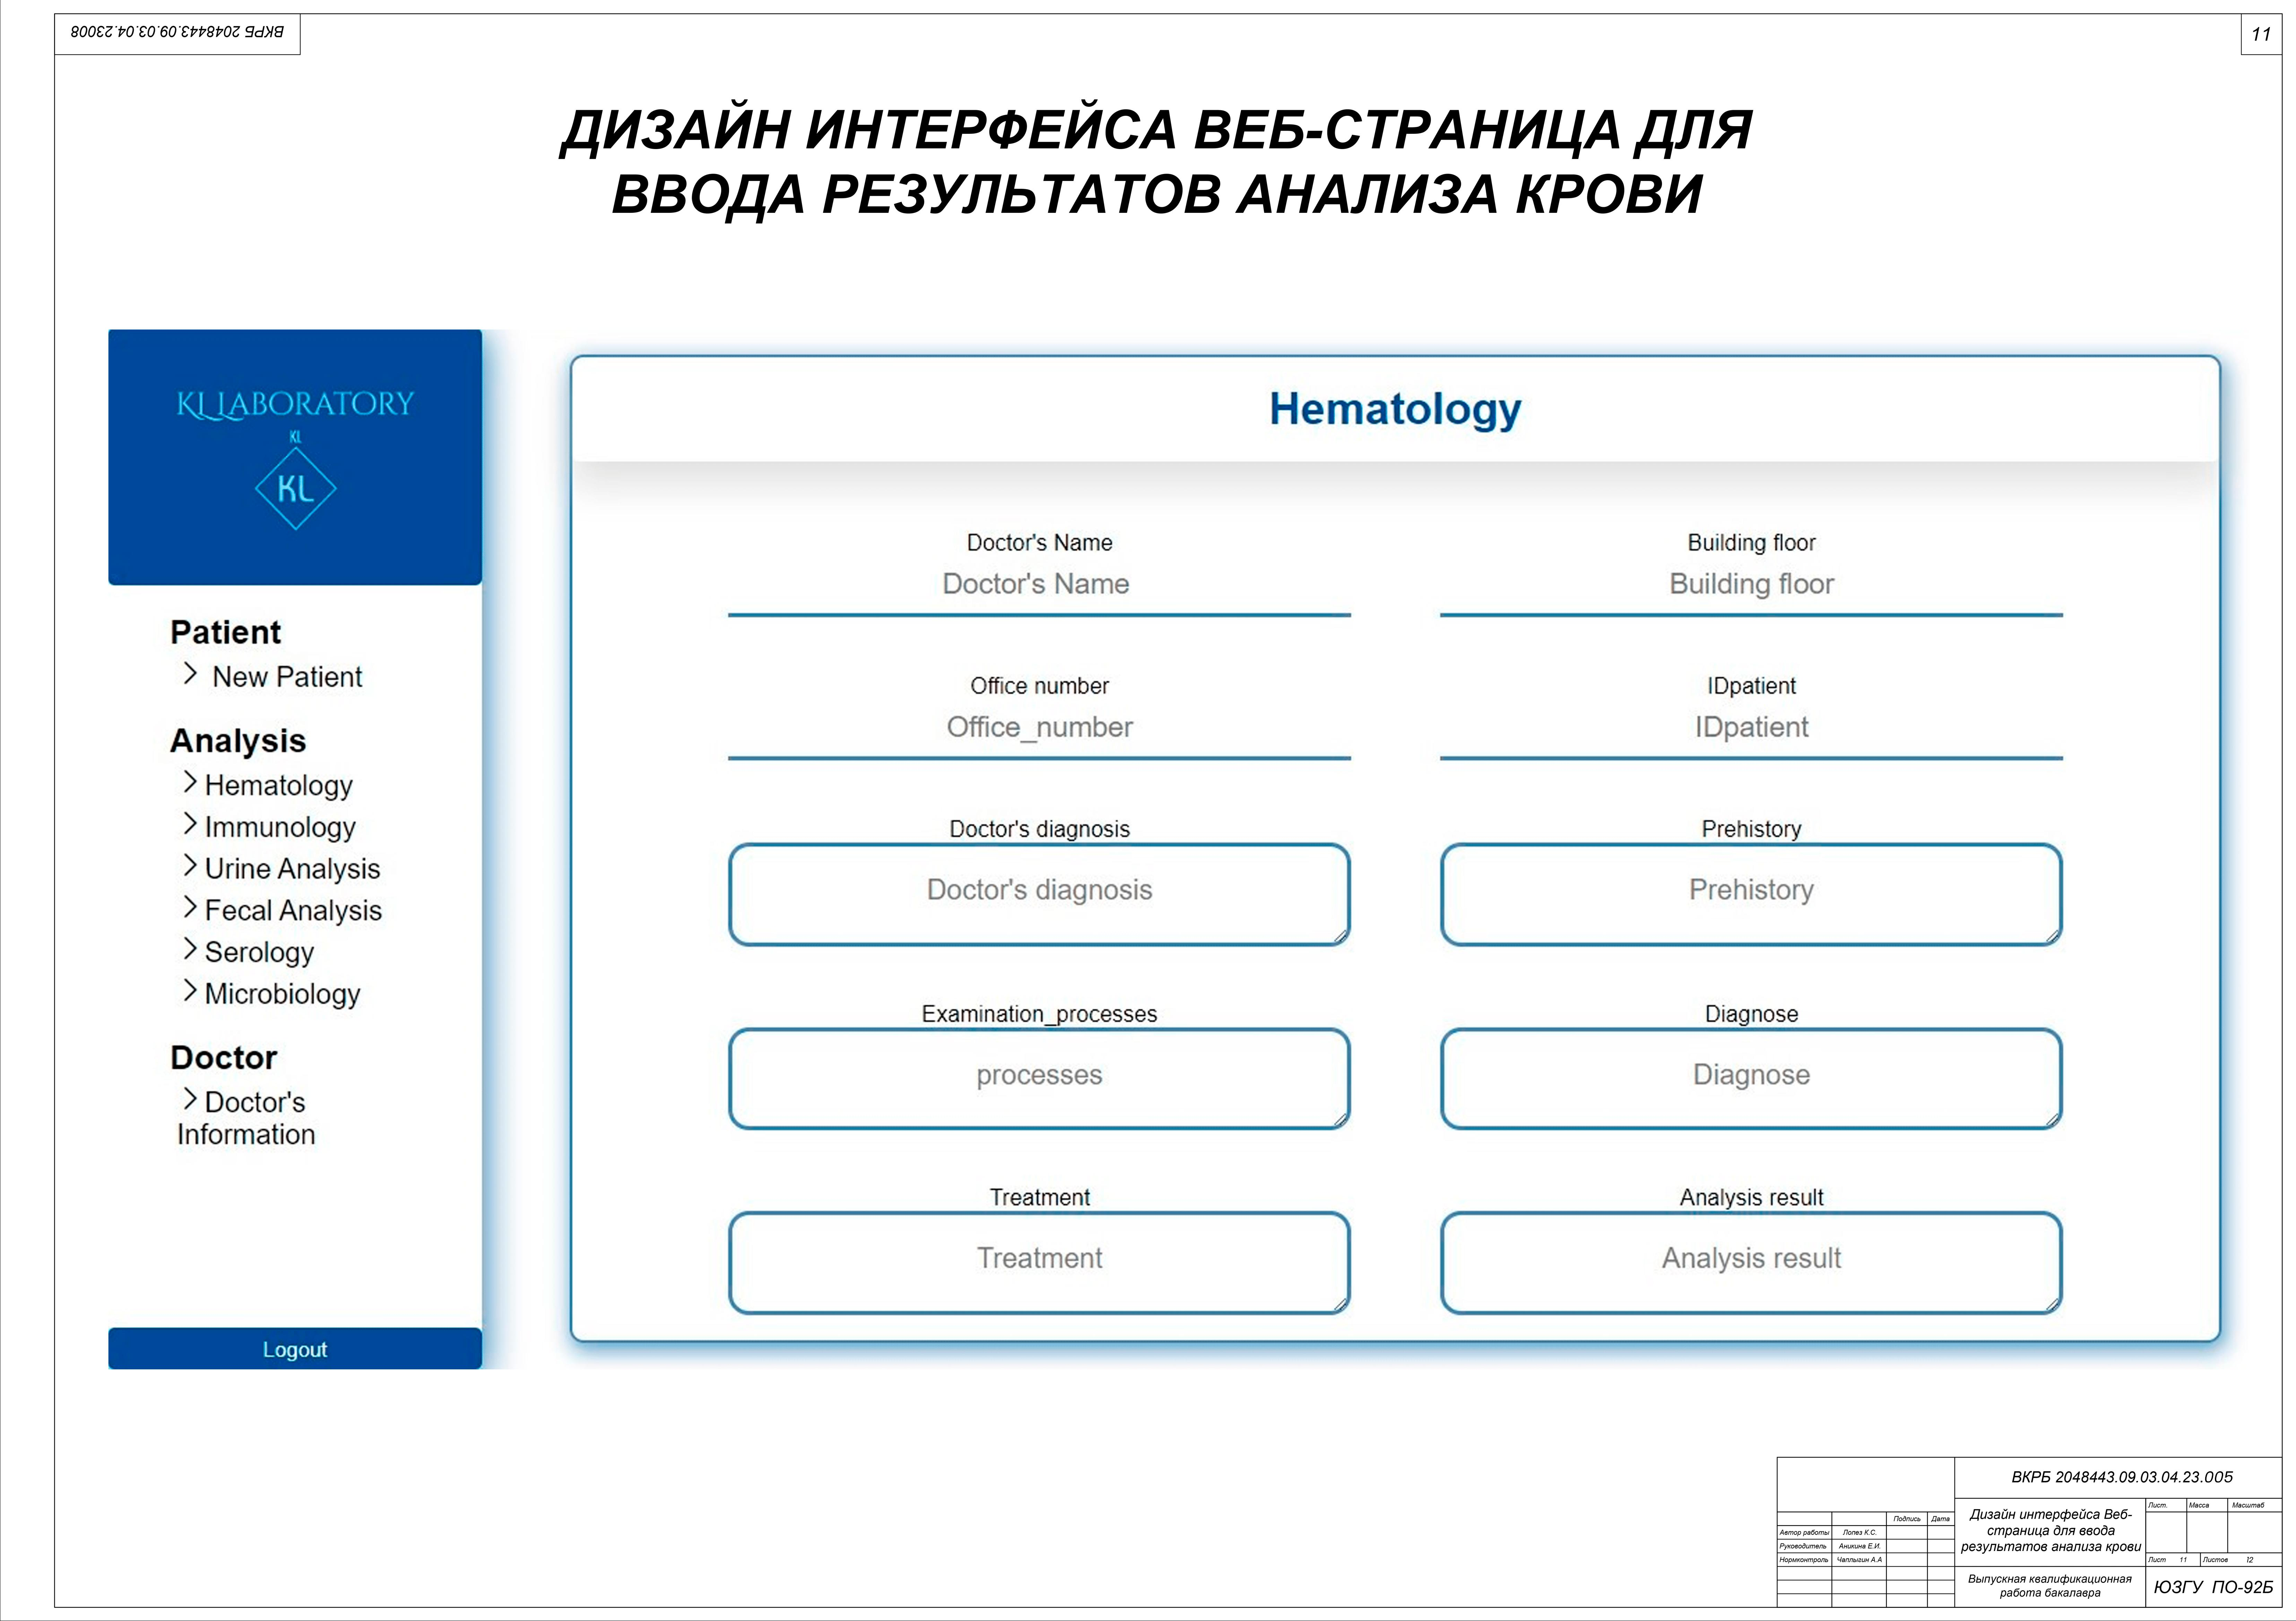
\includegraphics[width=1.3\linewidth]{плакат11.png}
	\end{adjustbox}
	\label{pl11:image}      
\end{figure}

\begin{figure}
	\begin{adjustbox}{addcode={\begin{minipage}{\width}}{\caption{%
						Заключение
			}\end{minipage}},rotate=90,center}
		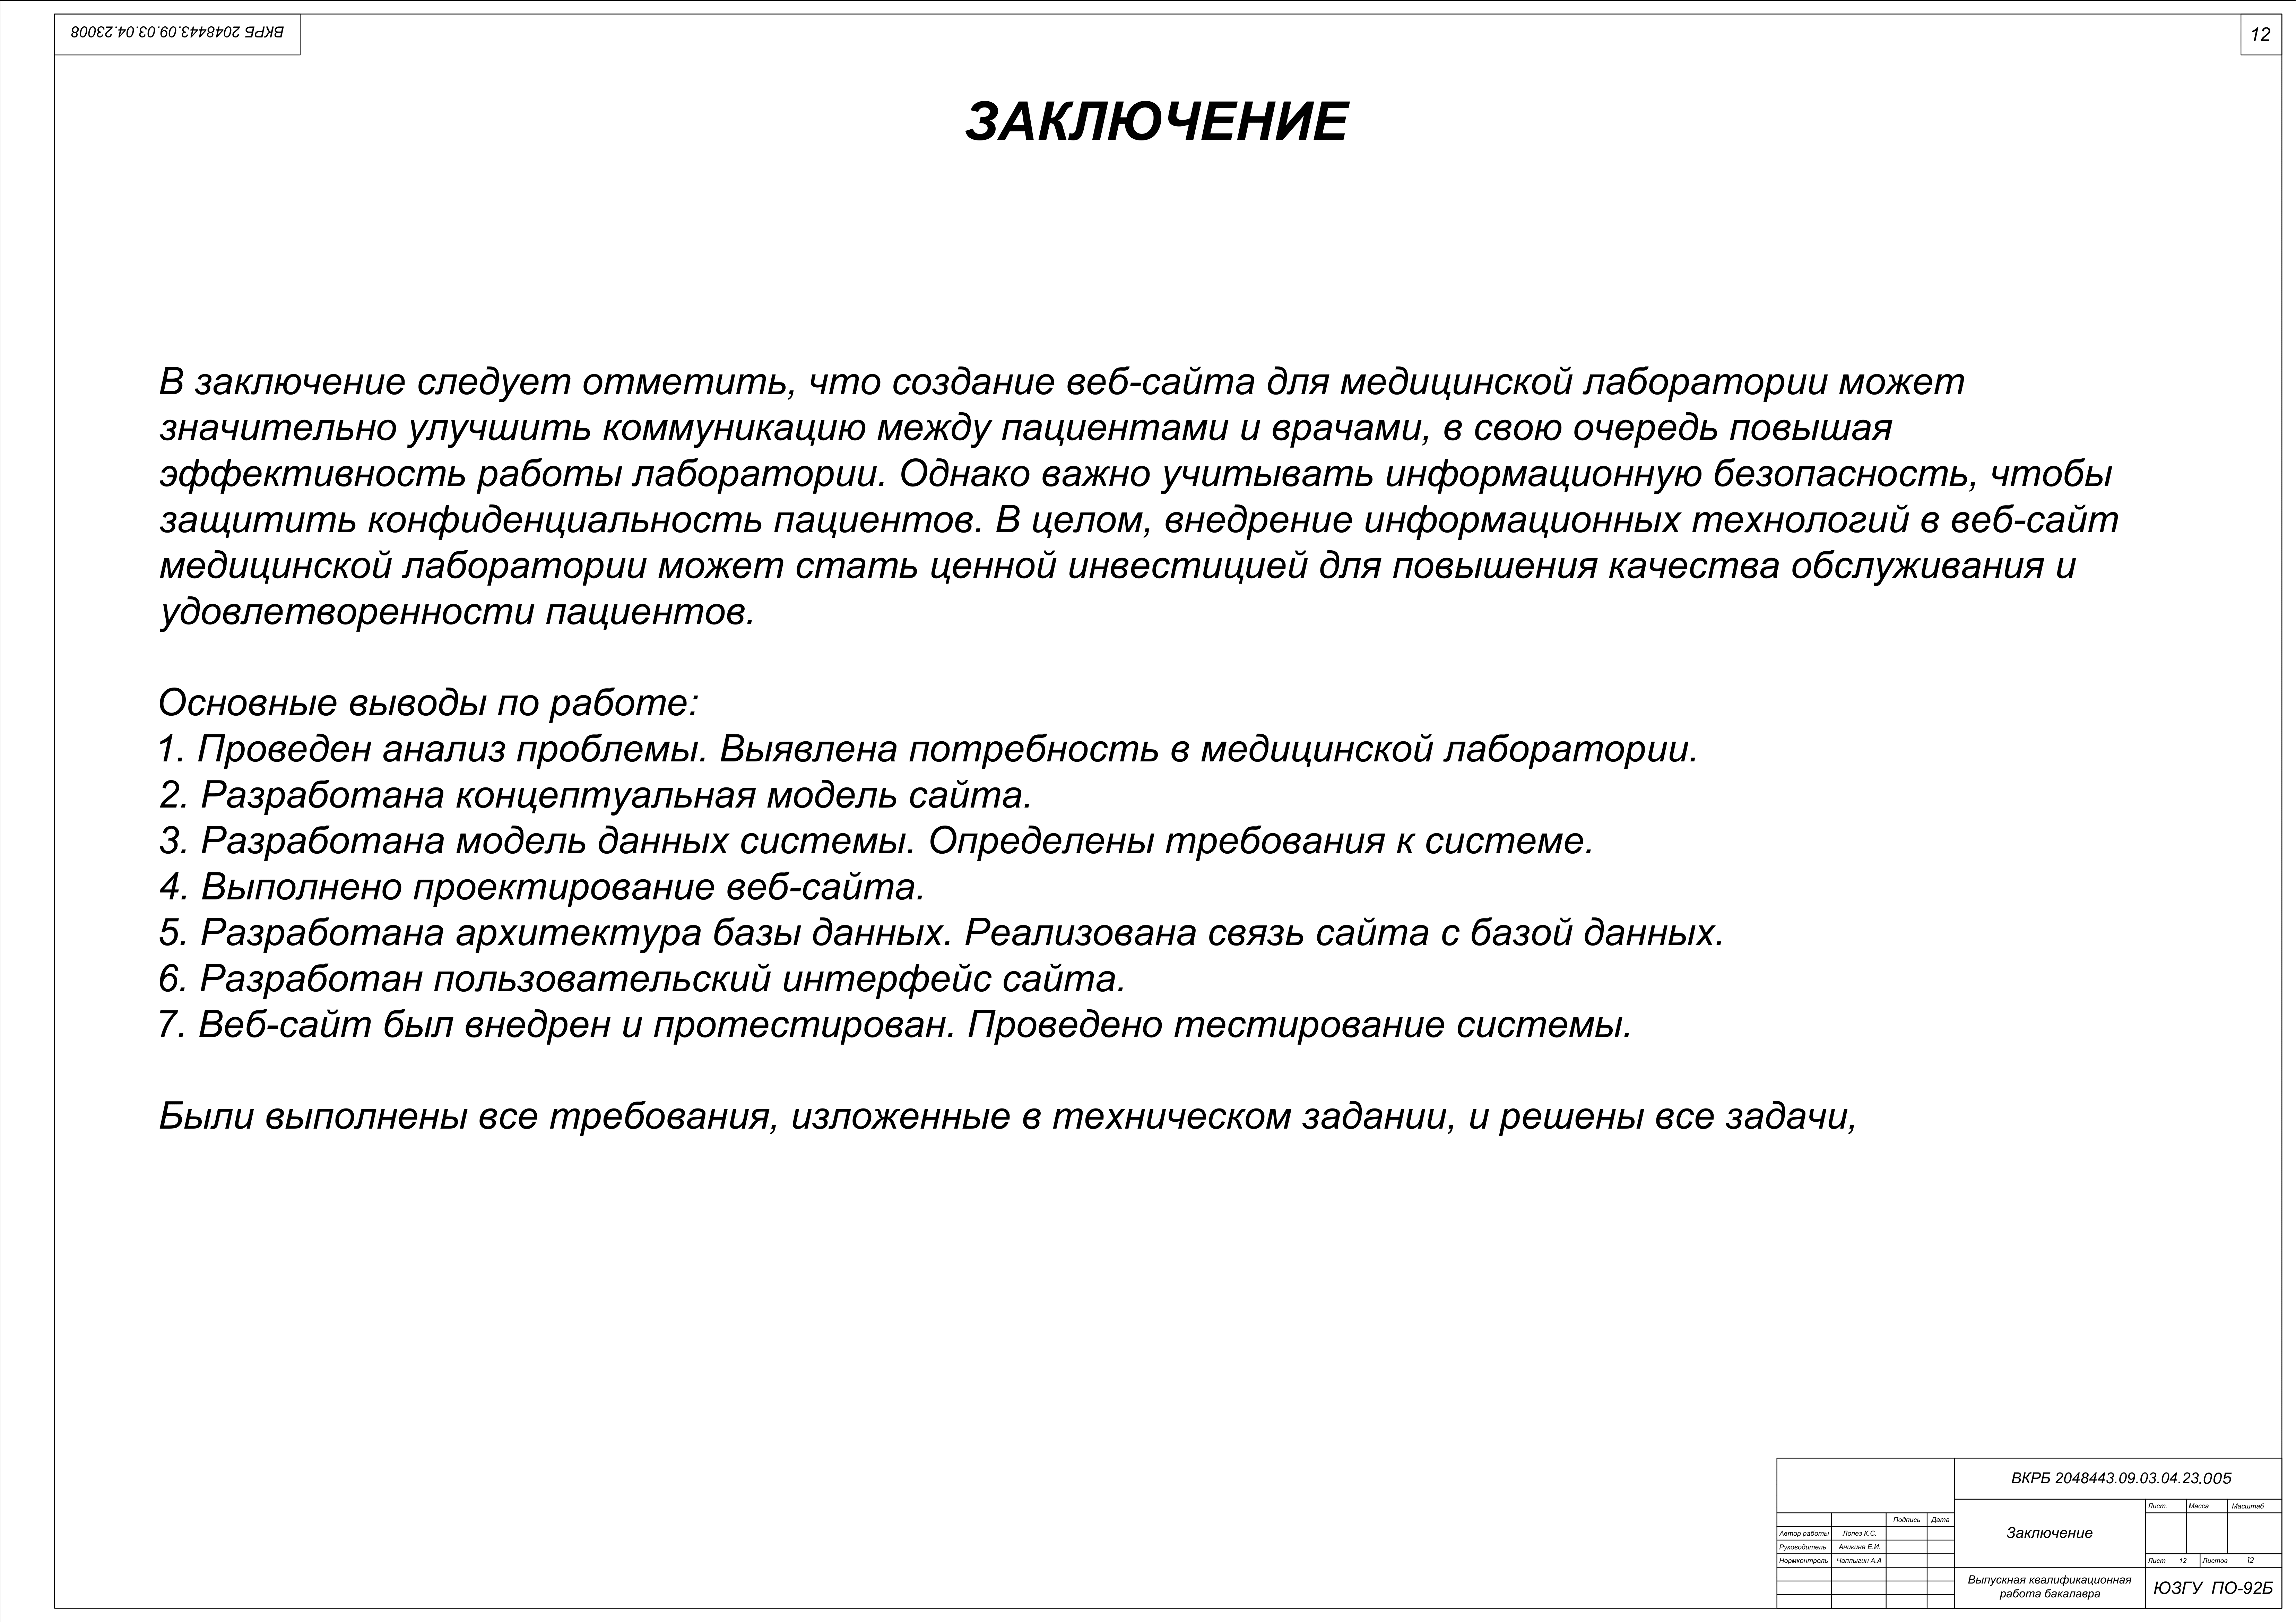
\includegraphics[width=1.3\linewidth]{плакат12.png}
	\end{adjustbox}
	\label{pl12:image}      
\end{figure}